\documentclass[oneside, 12pt]{book}
\usepackage{amsmath, amsthm, amssymb, url,graphicx}
\usepackage{makeidx}  % allows for indexgeneration
\usepackage{llncsdoc}
\usepackage{algorithmic}
\usepackage{amssymb}
\usepackage{graphicx}
\usepackage{wrapfig}
\usepackage{cite}
\usepackage{amsmath}
\usepackage[usenames,dvipsnames]{xcolor}
\usepackage[parfill]{parskip} 
\usepackage{float}
\usepackage{caption}
\usepackage[utf8]{inputenc}
\usepackage{combelow}% provides \cb to place comma below character

\usepackage{newunicodechar}
\newunicodechar{ș}{\cb{s}}
\newunicodechar{ț}{\cb{t}}

\newunicodechar{Ș}{\cb{S}}
\newunicodechar{Ț}{\cb{S}}

\title{Protocale Criptografice de Grup}
\author{Dragoș Alin Rotaru}
\date{2015}

\renewcommand{\chaptername}{Capitolul}
\renewcommand\contentsname{Cuprins}
\renewcommand{\bibname}{Referinţe}
\renewcommand{\figurename}{Figura}
\newcommand{\Mod}[1]{\ (\text{mod}\ #1)}
\newcommand{\todo}[1]{{\color{red}{TODO #1}}}

\newtheorem{implicatie}{\textbf{Implicața}}[section]
\newtheorem{observatie}{\textbf{Observația}}[section]
\newtheorem{definitie}{\textbf{Definiția}}[section]
\newtheorem{teorema}{\textbf{Teorema}}[section]
\newtheorem{lema}{\textbf{Lema}}[section]
%\def\examplename{Exemplul}

\newtheorem{exemplu}{\textbf{Exemplu}}[section]
 
\begin{document}
%  de titlu
\thispagestyle{empty}

\begin{center}
\centerline{\bf UNIVERSITATEA BUCUREȘTI}
\centerline{\bf FACULTATEA DE MATEMATICĂ ȘI INFORMATICĂ}

\end{center}
\vspace{4.5cm}

\centerline{\huge \bf Protocoale Criptografice de Grup}

\vspace{0.5cm}

\centerline{\large \bf Lucrare de Licență}

\vspace{3.5cm}

\begin{flushleft}
{\Large \textit{Coordonator:}\vspace{0.2cm}}

{\Large Lect.dr. Ruxandra F. Olimid}
\end{flushleft}

\vspace{1cm}
\begin{flushright}
{\Large \textit{Student:}\vspace{0.2cm}}

{\Large Dragoș Alin Rotaru}
\end{flushright}


\vspace{2cm}

\centerline{\bf BUCUREȘTI}

\centerline{\bf 2015}

\chapter*{Abstract}

\hspace*{5mm} Criptografia modernă se găsește pretutindeni în viața de zi cu zi de la ATM-uri, cartele telefonice la protocoale de autentificare, licitații electronice sau bani digitali, luând amploare o dată cu apariția sistemelor cu cheie publică. O definiție potrivită este \textit{studiul științific al tehnicilor pentru a securiza informația digitală, tranzacțiile și calculul distribuit} \cite{Katz:2007}. În cadrul criptografiei există primitive multiple care stau la baza tutoror protocoalelor precum: semnături digitale, vot electronic, scheme de partajare, schimbul sigur de chei. Un rol important îl deține criptografia de grup, care permite definirea și analiza securității unor protocoale la care iau parte mai mult de 2 participanți (vot elecronic, semnături de grup, partajarea de secrete).

\hspace*{5mm}Păstrarea confidențialității și redundanței datelor pe perioade lungi de timp reprezintă o sarcină dificilă din cauza multiplelor probleme care pot apărea precum atacuri, erori umane, defecțiunea unor componente hardware sau dezastre naturale \cite{SGMV:2009}. Problemele sunt cu atât mai actuale astăzi, când organizațiile își păstrează datele în cloud pentru scăderea costurilor necesare întreținerii unui centru propriu de date (datacenter), deci informațiile sunt stocate și procesate în afara unui control fizic al roprietarului.

\hspace*{5mm}Lucrarea de față analizează câteva dintre primitivele criptografice prezentând protocoale construite pe baza lor precum şi contribuţii personale în dezvoltarea lor \cite{RD:2014, RD:2015}. În final introducem o arhitectură implementată cu ajutorul schemelor de partajare, eliminând astfel câteva vulnerabilități prezente la sistemele descrise anterior.


%------------------------------------------------------------------------------------------
%------------------------------------------------------------------------------------------
%------------------------------------------------------------------------------------------
%------------------------------------------------------------------------------------------
%------------------------------------------------------------------------------------------
%------------------------------------------------------------------------------------------
%------------------------------------------------------------------------------------------
%------------------------------------------------------------------------------------------
%------------------------------------------------------------------------------------------
%------------------------------------------------------------------------------------------
%------------------------------------------------------------------------------------------
%------------------------------------------------------------------------------------------
%------------------------------------------------------------------------------------------
%------------------------------------------------------------------------------------------

\setcounter{tocdepth}{2}
\tableofcontents



%------------------------------------------------------------------------------------------
%------------------------------------------------------------------------------------------
%------------------------------------------------------------------------------------------
%------------------------------------------------------------------------------------------
%------------------------------------------------------------------------------------------
%------------------------------------------------------------------------------------------
%------------------------------------------------------------------------------------------
%------------------------------------------------------------------------------------------
%------------------------------------------------------------------------------------------
%------------------------------------------------------------------------------------------
%------------------------------------------------------------------------------------------
%------------------------------------------------------------------------------------------
%------------------------------------------------------------------------------------------
%------------------------------------------------------------------------------------------



% 					Structura
%------------------------------------------------------------------------------------------
%------------------------------------------------------------------------------------------
%------------------------------------------------------------------------------------------
%------------------------------------------------------------------------------------------
%------------------------------------------------------------------------------------------

\chapter*{Introducere şi organizarea lucrării}
\addcontentsline{toc}{chapter}{Structură}

\begin{itemize}
	%\item Secțiunea {\ref{sec:intro}} descrie pe scurt obiectul de studiu.
	\item \todo{Completeaza descrierea}
	\item Secțiunea {\ref{sec:splitting_schemes}} oferă o scurtă introducere în domeniul schemelor de partajare și descrie în detaliu construcțiile care vor fi folosite în secțiunile următoare.
	\item Secțiunea {\ref{sec:long_term_systems_full}} conține cerințele pe care trebuie să le îndeplinească un sistem de stocare de lunga durată și compară sistemele de stocare de lungă durată care utilizează criptarea cu sistemele de stocare bazate pe scheme de partajare a secretelor. De asemenea, sunt descrise câteva sisteme considerate relevante pentru întelegerea contribuțiilor până în prezent.
	\item Secțiunea {\ref{sec:desc_alouneh}} introduce un sistem de stocare criptanalizat.
	\item Secțiunea {\ref{sec:alouneh_contributions}} conține contribuțiile de cercetare, punând în evidență problemele cauzate de determinismul sistemului introdus în Secțiunea {\ref{sec:desc_alouneh}}.
\end{itemize}





%------------------------------------------------------------------------------------------
%------------------------------------------------------------------------------------------
%------------------------------------------------------------------------------------------
%------------------------------------------------------------------------------------------
%------------------------------------------------------------------------------------------




%------------------------------------------------------------------------------------------
%------------------------------------------------------------------------------------------
%------------------------------------------------------------------------------------------
%------------------------------------------------------------------------------------------
%------------------------------------------------------------------------------------------
%------------------------------------------------------------------------------------------
%------------------------------------------------------------------------------------------
%------------------------------------------------------------------------------------------
%------------------------------------------------------------------------------------------
%------------------------------------------------------------------------------------------
%------------------------------------------------------------------------------------------
%------------------------------------------------------------------------------------------
%------------------------------------------------------------------------------------------
%------------------------------------------------------------------------------------------

\section{Introducere + Motivatie - deocamdata text reciclabil}
\label{sec:intro}

Termenul de criptografie este definit in dicționarul Oxford ca fiind \textit{arta de a scrie și a rezolva coduri}.
Criptografia modernă s-a desprins de cea clasica în jurul anilor '80, motivând implementarea rigurozității matematice pentru definirea construcțiilor criptografice. Aceasta pentru ca în anii anteriori, experiența a dovedit nesiguranța metodelor de criptare, criptanaliza lor fiind uneori trivială (cifrul lui Cezar, Vigenere) sau uneori atinsă cu ceva mai mult efort precum Enigma și alte metode din cel de-al doilea război mondial.

Schemele de partajare sunt utilizate în aplicații precum: protejarea și recuperarea cheilor criptografice, vot electronic, certificate distribuite unor autorități, licitații on-line sau sisteme de stocare de lungă durată. \cite{Martin:2008}

O schemă de partajare reprezintă o metodă de a distribui un secret unor participanți, oferind fiecărui participant o componentă (share) astfel încât doar o submulțime de participanți pot recupera secretul inițial.

Cum volumul de datelor electronice este în continuă creștere, necesitatea stocării sigure a devenit extrem de necesară.

Date sensibile trebuie menținute secrete, câteodată pentru lungi perioade de timp (zeci de ani). Exemple includ informații militare, documete legale sau dosare medicale: informațiile militare pot fi clasificate zeci de ani, un testament trebuie menținut secret până la deschiderea sa oficială, un dosar medical necesită păstrare sigură (cel puțin) pe toată durata vieții pacientului.



%----------------------------------------------------------------
%----------------------------------------------------------------
%----------------------------------------------------------------
%----------------------------------------------------------------






%------------------------------------------------------------------------------------------
%------------------------------------------------------------------------------------------
%------------------------------------------------------------------------------------------
%------------------------------------------------------------------------------------------
%------------------------------------------------------------------------------------------
%------------------------------------------------------------------------------------------
%------------------------------------------------------------------------------------------
%------------------------------------------------------------------------------------------
%------------------------------------------------------------------------------------------
%------------------------------------------------------------------------------------------
%------------------------------------------------------------------------------------------
%------------------------------------------------------------------------------------------
%------------------------------------------------------------------------------------------
%------------------------------------------------------------------------------------------

\chapter{Funcții Pseudoaleatoare}
\label{cha:prf}

\section{Introducere}

O funcţie pseudoaleatoare (PRF) $F : \mathcal{K} \times \mathcal{X} \rightarrow \mathcal{Y}$ este un algoritm polinomial determinist definit pe mulţimea cheilor $\mathcal{K}$ unde $\mathcal{X}$, $\mathcal{Y}$ reprezintă domeniul, respectiv codomeniul lui $F$.
Primele construcţii au fost definite în $1986$ pornind de la un PRG (generator pseudoaleator) sigur \cite{goldreich1986construct}. Această primitivă este folosită în special pentru generarea de chei în protocoale actuale precum TLS (fostul SSL) \cite{dierks2008transport}.

Un caz particular de PRF în care $\mathcal{Y} = \mathcal{X}$ şi $F$ este bijectivă, sunt permutările pseudoaleatoare (PRP): AES, 3DES, având proprietatea utilă de a admite inversă. %as putea un nume mai bun, nu chiar inversabilitate

Intuitiv, funcţia $F$ poate fi evaluată eficient (în timp polinomial) în toate punctele $x \in \mathcal{X}$ din momentul în care o cheie $k \in \mathcal{K}$ este fixată. 
Din punct de vedere al securității, un adversar PPT (timp probabilistic polinomial) $\mathcal{A}$ nu poate face diferența între o instanţă aleatoare $F(k, \cdot)$, $k \in \mathcal{K}$ şi o funcție aleasă aleator din toate funcţiile posibile având domeniul $\mathcal{X}$, codomeniul $\mathcal{Y}$.

%----------------------------------------------------------------
%----------------------------------------------------------------
%----------------------------------------------------------------
%----------------------------------------------------------------

\section{Definiții de Securitate}
\label{subsec:prf-security}

În procesul formalizării noţiunii de securitate \textit{adaptivă} a unei funcții PRF $F$, vom avea în vedere un adversar PPT $\mathcal{A}$. În definiție sunt prezentate $2$ experimente cu adversarul $\mathcal{A}$: $EXP(b))$, $b \leftarrow ^ R \{0,1\}$, iar avantajul lui va consta în abilitatea de a le distinge. Notăm cu $s \leftarrow^R S$ faptul că $s$ este ales în mod aleator uniform din mulţimea $S$. 

La începutul experimentului este apelată funcția $Setup(1^\lambda)$ care primește la intrare un parametru de securitate $\lambda$ și întoarce o cheie secretă $k \leftarrow^R \mathcal{K}$. Fie $V, C \subseteq X$, $2$ mulțimi de puncte (inițial vide) pentru care $\mathcal{A}$ cunoaște valorile $F(k, \cdot)$ trimise la $\mathsf{F.eval}$, respectiv la $\mathsf{F.challenge}$. De asemenea, $\mathcal{A}$ are acces la $2$ tipuri de oracole:
\begin{itemize}
	\item $\mathsf{F.eval}$: pentru un $x \in \mathcal{X}$ întoarce $F(k, x)$ dacă $x \not \in C$ și actualizează mulțimea $V \leftarrow V \cup x$, altfel $\bot$ $(\not \in \mathcal{Y})$.
	\item $\mathsf{F.challenge}$: pentru un $x \not \in V$ întoarce $F(k, x)$ dacă $b = 0$ și $y \leftarrow^R \mathcal{Y}$ dacă $b = 1$ iar $C \leftarrow C \cup x$. 
\end{itemize}
La finalul experimentului, $\mathcal{A}$ întoarce o valoare $b' \in \{0, 1\}$.

Fie $W_b$ evenimentul ca în urma eperimentului $EXP(b)$, $b'$ să fie $1$ la sfârșitul jocului. Notăm cu $AdvPRF_{\mathcal{A},F}(\lambda) = |Pr[W_0] - Pr[W_1]|$ avantajul lui $A$.

\begin{definitie}
	O funcție PRF $F$ este sigură dacă pentru orice adversar PPT A, $AdvPRF_{\mathcal{A},F}(\lambda)$ este o funcție neglijabilă.
\end{definitie}


\section{Funcții Pseudoaleatoare Constrânse}
\label{subsec:cprf}

O funcție cPRF (pseudoaleatoare constrânsă) $F : \mathcal{K} \times \mathcal{X} \rightarrow \mathcal{Y}$ este o funcție PRF care deține \textit{chei de constrângere} ce permit evaluarea funcției $F$ în subdomenii $S \subseteq 2^{\mathcal{X}}$ menținând proprietățile de securitate ale funcțiilor PRF.

\begin{definitie}
\label{def:cprf}
	O funcție PRF $F : \mathcal{K} \times \mathcal{X} \rightarrow \mathcal{Y}$ este constrânsă la o mulțime $\mathcal{S} \subseteq 2^{\mathcal{X}}$ dacă există o mulțime adițională de chei $\mathcal{K}_c$ și $2$ algoritmi:
	\begin{itemize}
		\item $\mathsf{F.constrain(k, S)}$: un algoritm nedeterminist care pentru o cheie $k \in \mathcal{K}_c$ și o mulțime $S \subseteq \mathcal{S}$ întoarce o cheie $k_s \in \mathcal{K}_c$ pentru care se poate face evaluarea lui $F(k, x)$ pentru orice $x \in S$.
		\item $\mathsf{F.eval(k_s, x)}$: un algoritm determinist care pentru o cheie $k_s \in \mathcal{K}_c$ și un punct $x \in \mathcal{X}$ întoarce $F(k, x)$  $\mbox{dacă} \hspace{.1in} x \in S$, sau $\bot$ $(\not \in \mathcal{Y})$ $\mbox{dacă} \hspace{.1in} x \notin S$
	\end{itemize}
\end{definitie}

Alte construcții pe baza cPRF definite în \cite{boneh:2013constrained} și care vor fi folosite ulterior sunt: \textit{stânga/dreapta PRF} - funcții cPRF ce admit evaluarea lor având partea stângă a domeniului fixată; \textit{bit-fixate PRF} - funcții cPRF care pot fi evaluate în domenii corespunzătoare unei expresii având unii biți fixați. Autorii \cite{boneh:2013constrained} menționează că aceste construcții sunt posibile în contextul funcțiilor multiliniare iar problema devine mai interesantă (deocamdată nerezolvată) în contextul LWE \cite{regev2009lattices}. 

\begin{definitie}
	Fie o funcție $F: \mathcal{K} \times \mathcal{X}^2 \rightarrow \mathcal{Y}$ PRF. $\forall v \in \mathcal{X}$ o funcție stânga/dreapta admite $2$ chei de constrângere ${k_v}^L$ și ${k_v}^R$ ce permit evaluarea funcției $F$ în toate punctele $(v, x) \in \mathcal{X}^2$, respectiv $(x, v) \in \mathcal{X}^2$. Notăm această funcție cPRF stânga/dreapta cu $PRF^{L/R}$.
\end{definitie}

\begin{definitie}
	Fie o funcție $F: \mathcal{K} \times {\{0, 1\}}^n \rightarrow \mathcal{Y}$ PRF. $\forall v \in {\{0, 1, ? \}}^n$ o funcție bit-fixată admite o cheie de constrângere $k_v$ ce permite evaluarea funcției $F$ în toate punctele $x \in \{0,1\}^n$ ce satisfac modelul lui $v$.
	Notăm această funcție cPRF bit-fixată cu $PRF^{bf}$.
\end{definitie}

Noțiunea de securitate pentru cPRF \cite{boneh:2013constrained} este asemănătoare cu cea pentru PRF: $2$ experimente $EXP(0), EXP(1)$, doar că în acest caz este necesară existența unui oracol $F.constrain$ pentru a permite adversarului să interogheze $F$ conform definiției \ref{def:cprf}.

La începutul fiecărui experiment este apelată funcția $Setup(\lambda)$ care întoarce o cheie secretă $k \leftarrow^R \mathcal{K}$. Inițial mulțimile $V, C \subseteq \mathcal{X}$ sunt vide iar adversarul $\mathcal{A}$ are acces la $3$ oracole:
\begin{itemize}
	\item $\mathsf{F.eval}$: pentru un $x \in \mathcal{X}$ întoarce $F(k, x)$ dacă $x \not \in C$ și actualizează mulțimea $V \leftarrow V \cup x$, altfel $\bot$;
	\item $\mathsf{F.constrain}$: pentru o mulțime $S \in \mathcal{S}$ întoarce $F.constrain(k, S)$ dacă $S \cap C = \emptyset$ și actualizează mulțimea $V = V \cup x$, altfel $\bot$;
	\item $\mathsf{F.challenge}$: pentru un $x \not \in V$ întoarce $F(k, x)$ dacă $b = 0$ și $y \leftarrow^R \mathcal{Y}$ dacă $b = 1$ iar $C \leftarrow C \cup x$;
\end{itemize}

La finalul experimentului, $\mathcal{A}$ întoarce o valoare $b' \in \{0, 1\}$.

Fie $W_b$ evenimentul ca în urma eperimentului $EXP(b)$, $b'$ să fie $1$ la sfârșitul jocului. Notăm cu $AdvPRF_{\mathcal{A},F}(\lambda) = |Pr[W_0] - Pr[W_1]|$ avantajul lui $A$.

\begin{definitie}
	O funcție cPRF $F$ este sigură dacă pentru orice adversar PPT $\mathcal{A}$, $AdvPRF_{\mathcal{A},F}(\lambda)$ este o funcție neglijabilă.
\end{definitie}


%------------------------------------------------------------------------------------------
%------------------------------------------------------------------------------------------
%------------------------------------------------------------------------------------------
%------------------------------------------------------------------------------------------
%------------------------------------------------------------------------------------------
%------------------------------------------------------------------------------------------
%------------------------------------------------------------------------------------------
%------------------------------------------------------------------------------------------
%------------------------------------------------------------------------------------------
%------------------------------------------------------------------------------------------
%------------------------------------------------------------------------------------------
%------------------------------------------------------------------------------------------
%------------------------------------------------------------------------------------------
%------------------------------------------------------------------------------------------

\chapter{NIKE}
\label{cha:nike}

NIKE (Non Interactive Key Exchange - schimb de chei non-interactiv) reprezintă o primitivă criptografică importantă în care o mulțime de participanți pot stabili de comun acord o cheie comună fără ca aceștia să fie on-line în același timp. Un exemplu des întâlnit în zilele noastre este schimbul de chei Diffie-Hellman \cite{diffie1976new}. Construcția a fost apoi extinsă la $3$ persoane de Joux folosind funcții biliniare \cite{joux2000one} iar Boneh și Silverberg au generalizat la $n$ persoane (multi-party) bazându-se pe funcții multi-liniare \cite{boneh:2003applications}.

%------------------------------------------------------------------------------------------
%------------------------------------------------------------------------------------------
%------------------------------------------------------------------------------------------
%------------------------------------------------------------------------------------------
%------------------------------------------------------------------------------------------
\section{ID-NIKE}
\label{sec:id-nike}

Criptografia bazată pe identitatea participanților a fost introdusă de Shamir în anul 1985 \cite{shamir:1985identity}. Aceasta presupune folosirea identității (email, nume, stradă), informație care îl identifică pe un utilizator într-un mod unic, fără să genereze o pereche de cheie publică, secretă. Principalul dezavantaj este necesitatea unei terțe autorizată care să administreze generarea de chei secrete, însă avantajul este utilizarea de mai puține resurse din partea participanților.

Așadar criptografia bazată pe ID este ideală într-un mediu în care utilizatorii dețin resurse computaționale limitate (rețea de routere).

ID-NIKE combină principiile oferite de NIKE cu ID-urile participanților.

\begin{definitie}
 	Formal, ID-NIKE constă în $3$ algoritmi:
	\begin{itemize}
		\item $Setup(\lambda)$: primește ca date de intrare parametrul de securitate $\lambda$ și întoarce o cheie secretă $msk$ împreună cu parametrii publici $params$;
		\item $Extract(msk, id_i)$: primește ca date de intrare cheia master secretă $msk$, identitatea $id_i \in \mathcal{ID}$ și întoarce cheia privată $sk_{id_i}$;
		\item $KeyGen(params, sk_{id_i}, id_j)$: primește ca date de intrare parametrii publici $params$, o cheie secretă $sk_{id_i}$, o identitate $id_j \neq id_i$ și întoarce cheia comună $k_{id_i, id_j}$.
	\end{itemize}
\end{definitie}

%------------------------------------------------------------------------------------------
%------------------------------------------------------------------------------------------
\subsubsection{Corectitudine}
Este garantată dacă pentru orice pereche de participanți, $id_i, id_j$ $\in \mathcal{ID}$, $id_i \neq id_j$ $KeyGen(params, sk_{id_i}, id_j)$ $=$ $KeyGen(params, sk_{id_j}, id_i)$. 

%------------------------------------------------------------------------------------------
%------------------------------------------------------------------------------------------
\subsubsection{Securitate}
\label{subsub:nike-security}

Amintim definiția de securitate adaptivă pentru ID-NIKE din \cite{paterson:2009relations}.

Fie $EXP(b)$, $b \leftarrow^R \{0,1\}$, două experimente cu un adeversar $PPT$ $\mathcal{A}$. La începutul fiecărui experiment $EXP(b)$ se execută $Setup(\lambda)$ oferind adversarului $\mathcal{A}$ $params$ și menținând cheia master $msk$ privată. $\mathcal{A}$ are acces la $3$ oracole:
\begin{itemize}
	\item $Ext(id_i)$: primește ca date de intrare o identitate $id_i$, apelează $Extract(msk, id_i)$ și întoarce $sk_{id_i}$;
	\item $Rev(id_i, id_j)$: primește ca date de intrare $2$ identități $id_i, id_j$, $id_i \neq id_j$, apelează funcția $Extract(msk, id_i)$ și întoarce cheia comună $k_{id_i, id_j}$ din $KeyGen(params, sk_{id_i}, id_j)$;
	\item $Test(id_i, id_j)$: primește ca date de intrare $2$ identități $id_i, id_j$, $id_i \neq id_j$. Dacă $b = 0$ atunci întoarce $Rev(id_i, id_j)$, altfel întoarce $sk_{id_i, id_j} \leftarrow^R \mathcal{SKS}$ unde cu $\mathcal{SKS}$ am notat spațiul de chei comune posibile.
\end{itemize}

Pentru a elimina situația în care adersarul $\mathcal{A}$ câștigă trivial, acestuia nu îi este permis să interogheze $Ext$ pentru o identitate în $Test$, precum și faptul că toate interogările $Rev$ și $Test$ să fie distincte.

La finalul experimentului, $\mathcal{A}$ întoarce o valoare $b' \in \{0, 1\}$.

Fie $W_b$ evenimentul ca în urma eperimentului $EXP(b)$, $b'$ să fie $1$ la sfârșitul jocului. Notăm cu $AdvKE_{\mathcal{A}}(\lambda) = |Pr[W_0] - Pr[W_1]|$ avantajul lui $A$.

\begin{definitie}
	ID-NIKE este adaptiv sigură dacă pentru orice adersar PPT, $\mathcal{A}$ funcția $AdvKE_{\mathcal{A}}(\lambda)$ este neglijabilă.
\end{definitie}

%------------------------------------------------------------------------------------------
%------------------------------------------------------------------------------------------
\subsection{Construcția Boneh-Waters (2013)}
\label{subsec:boneh-waters}
În figura \ref{fig:bw-nike} prezentăm construcția Boneh-Waters bazată pe funcții constrânse stânga/dreapta \cite{boneh:2013constrained}.

\begin{figure*}[h!]

\begin{tabular}{|p{\textwidth}|}
\hline

\\
\hspace{.1in}
$\mathsf{Setup}(\lambda)$: Fie $F : \mathcal{K} \times \mathcal{X}^2 \rightarrow \mathcal{Y}$ o funcție cPRF stânga/dreapta sigură, alege \\
	\hspace{.3in} în mod aleator $msk \leftarrow^R \mathcal{K}$ și întoarce parametrii publici $params$ \\ 
	\hspace{.3in} corespunzători funcției $F$; \\

\\
\hspace{.1in}
$\mathsf{Extract}(msk, id_i)$: calculează $\mathsf{F.constrain}(msk, \{(id_i, \cdot)\})$ pentru a obține $k^{L}_{id_i}$ \\
	\hspace{.3in} și $\mathsf{F.constrain}(msk, \{(\cdot, id_i)\})$ pentru a obține $k^{R}_{id_i}$, apoi \\ 
	\hspace{.3in} întoarce $sk_{id_i} = (k^{L}_{id_i},k^{R}_{id_i})$; \\

\\
\hspace{.1in}
$\mathsf{KeyGen}(params, sk_{id_i},id_j)$: întoarce $F(msk, (id_i, id_j))$ dacă $id_i < id_j$ și \\
	\hspace{.3in} $F(msk, (id_j, id_i))$ dacă $ id_i > id_j$ (în ordine lexicografică).

\\
\hline
\end{tabular}
\caption{Construcția Boneh-Waters \cite{boneh:2013constrained}}
\label{fig:bw-nike}
\end{figure*}

%------------------------------------------------------------------------------------------
%------------------------------------------------------------------------------------------
\subsubsection{Corectitudine}

Reiese din funcția cPRF stânga/dreapta. Fie $2$ participanți având identitățile $id_i, id_j$ cu $id_i < id_j$. Participantul cu $id_i$ folosește cheia $k^{L}_{id_i}$ iar cel cu $id_j$ cheia $k^{R}_{id_i}$. În acest moment $id_i$ poate calcula $F(msk, (id_i, \cdot))$ iar $id_j$, $F(msk, (\cdot, id_j))$ în acest mod stabilind cheia comună $F(msk, (id_i, id_j))$.

%------------------------------------------------------------------------------------------
%------------------------------------------------------------------------------------------
\subsubsection{Securitate}

Reiese din securitatea funcției cPRF stânga/dreapta. Dacă un adversar $\mathcal{B}$ împotriva unei funcții cPRF stânga/dreapta simulează perfect adeversarul $\mathcal{A}$ pentru construcția Boneh-Waters atunci demonstrația este completă. Așadar, luând în considerare cele $3$ oracole din \ref{subsub:nike-security}, în cazul in care $\mathcal{A}$ interoghează:
\begin{itemize}
	\item $Ext(id_i)$: $\mathcal{B}$ interoghează $\mathsf{F.constrain}$ pentru toate $S$ având valorile $(id_i, \cdot)$ și $(\cdot, id_i)$; întoarce rezultatul lui $\mathcal{A}$;
	\item $Rev(id_i, id_j)$: $\mathcal{B}$ interoghează $\mathsf{F.eval}$ pentru $(id_i, id_j)$ dacă $id_i < id_j$, altfel interoghează pentru $(id_j, id_i)$; întoarce rezultatul lui $\mathcal{A}$;
	\item $Test(id_i, id_j)$: $\mathcal{B}$ interoghează $\mathsf{F.challenge}$ și întoarce răspunsul lui $\mathcal{A}$.
\end{itemize}




%------------------------------------------------------------------------------------------
%------------------------------------------------------------------------------------------
%------------------------------------------------------------------------------------------
%------------------------------------------------------------------------------------------
%------------------------------------------------------------------------------------------
\section{Multi-Party ID-NIKE}
\label{subsec:multi-party-id}

Multi-Party (mai mulți membri) ID-NIKE reprezintă generalizarea protocolului ID-NIKE pentru cazul cu $n$ participanți $(n > 2)$. Mai întâi definim modelul de securitate pentru acest protocol după care introducem construcția multi-party bazată pe funcții cPRF bit-fixate din secțiunea \label{sec:multi-party-contributions} \cite{RD:2014}.

\begin{definitie}
	O schemă multi-party ID-NIKE este formată din $3$ algoritmi:
	\begin{itemize}
		\item $Setup(\lambda, n)$: primește ca date de intrare parametrul de securitate $\lambda$ și $n$, un număr întreg reprezentănd numarul de participanți; calculează cheia secretă master $msk$ și intoarce parametrii publici $params$;
		\item $Extract(msk, id_i)$: primește cheia secretă master $msk$, o identitate $id_i \in \mathcal{ID}$ și întoarce o cheie secretă $sk_{id_i}$;
		\item $KeyGen(params, sk_{id_i}, \{id_l\}_{l=1,\dots,n})$: primește parametrii publici $params$, $n$ identități distincte $id_1, id_2, \dots, id_n$, cheia secretă $sk_{id_i}$ a identității $id_i$ și întoarce cheia comună $sk_{id_1, id_2, \dots, id_n}$.
	\end{itemize}
\end{definitie}

\subsubsection{Corectitudine}
Este necesar ca toți participanții să obțină aceeași cheie; Pentru orice pereche $i, j, i \neq j$ și $n$ identități distincte $id_1, id_2, \dots, id_n$: $KeyGen(params, sk_{id_i}, \{id_l\}_{l=1,\dots,n})$ = $KeyGen(params, sk_{id_j}, \{id_l\}_{l=1,\dots,n})$.


%----------------------------Security Definition--------------------------------------------------

\subsubsection{Securitate}

Definiția de securitate este similară ca în cazul ID-NIKE. La începutul fiecărui experiment $EXP(b)$ se execută $Setup(\lambda, n)$ iar parmetrii $params$ se fac publici. Un adversar $\mathcal{A}$ are acces la $3$ tipuri de oracole:
\begin{itemize}
	\item $Ext(id_i)$: pentru o identitate $id_i$ apelează $Extract(msk,id_i)$ și întoarce $sk_{id_i}$;
	\item $Rev(id_1, id_2, \dots, id_n)$: pentru $n$ identități $id_1, id_2, \dots, id_n$ distincte, apelează $Extract(msk, id_i)$ pentru a afla $sk_{id_i}$; Întoarce $KeyGen(params$ $,sk_{id_i},$ $\{id_l\}_{l=1,\dots,n})$;
	\item $Test(id_1, id_2, \dots, id_n)$: dacă $b = 0$ întoarce $Rev(id_1, id_2, \dots, id_n)$; dacă $b = 1$ întoarce $sk_{id_1, id_2, \dots, id_n} \leftarrow^R \mathcal{SKS}$.
\end{itemize}

Pentru a elimina situația în care adersarul $\mathcal{A}$ câștigă trivial, acestuia nu îi este permis să interogheze $Ext$ pentru o identitate în $Test$, precum și faptul că toate interogările $Rev$ și $Test$ trebuie să fie distincte. La finalul experimentului, $\mathcal{A}$ întoarce o valoare $b' \in \{0, 1\}$.

Fie $W_b$ evenimentul ca în urma eperimentului $EXP(b)$, $b'$ să fie $1$ la sfârșitul jocului. Notăm cu $AdvKE_{\mathcal{A}, n}(\lambda) = |Pr[W_0] - Pr[W_1]|$ avantajul lui $A$.


\begin{definitie}
	Multi-party ID-NIKE este adaptiv sigură dacă pentru orice adersar PPT, $\mathcal{A}$ funcția $AdvKE_{\mathcal{A},n}(\lambda)$ este neglijabilă.
\end{definitie}

%----------------------------End of Security Definition-------------------------------------------
%------------------------------------------------------------------------------------------
%------------------------------------------------------------------------------------------
%------------------------------------------------------------------------------------------
%------------------------------------------------------------------------------------------
%------------------------------------------------------------------------------------------
\section{Contribuții}
\label{sec:multi-party-contributions}

Pornind de la construcția Boneh-Waters ID-NIKE extindem protocolul la o schemă având $n$ participanți, înlocuind funcția cPRF stânga/dreapta cu o funcție cPRF bit-fixată \cite{RD:2014}.

\begin{figure*}[h!]

\begin{tabular}{|p{\textwidth}|}
\hline

\\
\hspace{.1in}
$\mathsf{Setup}(\lambda, n)$: Fie $F : \mathcal{K} \times \mathcal{X}^n \rightarrow \mathcal{Y}$ o funcție cPRF bit-fixată sigură, alege \\
	\hspace{.3in} în mod aleator $msk \leftarrow^R \mathcal{K}$ și întoarce parametrii publici $params$ \\ 
	\hspace{.3in} corespunzători funcției $F$; \\
\\
\hspace{.1in}
$\mathsf{Extract}(msk, id_i)$: calculează: \\
	\hspace{.3in} $\mathsf{F.constrain}(msk, \{(id_i, \cdot, \dots, \cdot)\})$ pentru a obține $k^1_{id_i}$, \\
	\hspace{.3in} $\mathsf{F.constrain}(msk, \{(\cdot, id_i, \dots, \cdot)\})$ pentru a obține $k^2_{id_i}$ $\dots$ \\
	\hspace{.3in} $\mathsf{F.constrain}(msk, \{(\cdot, \dots, \cdot, id_i)\})$ pentru a obține $k^n_{id_i}$, \\
	\hspace{.3in} apoi întoarce $sk_{id_i} = (k^{1}_{id_i}, k^{2}_{id_i}, \dots, k^{n}_{id_i})$; \\
\\
\hspace{.1in}
$\mathsf{KeyGen}(params, sk_{id_i},\{id_l\}_{l=1,\dots,n})$: \\
	\hspace{.3in} întoarce $F(msk, (id_{\pi(1)}, id_{\pi(2)}, \dots, id_{\pi(N)}))$,\\
	\hspace{.3in} unde $id_{\pi(1)} < id_{\pi(2)} < \dots < id_{\pi(N)}$ (în ordine lexicografică).

\\
\hline
\end{tabular}
\caption{Construcția multi-party ID-NIKE \cite{RD:2014}}
\label{fig:our-construction}
\end{figure*}

%------------------------------------------------------------------------------------------
%------------------------------------------------------------------------------------------
\subsubsection{Corectitudine}
	Este garantată din construcția funcției cPRF bit-fixate. Pentru a obține cheia comună, participantul cu identitatea $id_i$ folosește $k^{\pi(i)}_{id_i}$ pentru a evalua funcția $F$.

%------------------------------------------------------------------------------------------
%------------------------------------------------------------------------------------------
\subsubsection{Securitate}
	Reiese din securitatea funcției cPRF bit-fixate. Dacă un adversar $\mathcal{B}$ împotriva unei funcții cPRF bit-fixate simulează perfect adeversarul $\mathcal{A}$ pentru multi-party ID-NIKE atunci demonstrația este completă. Așadar, luând în considerare cele $3$ oracole din \ref{subsub:nike-security}, în cazul in care $\mathcal{A}$ interoghează:
	\begin{itemize}
		\item $Ext(id_i)$: $\mathcal{B}$ interoghează $\mathsf{F.constrain}$ pentru toate punctele din domeniul $\mathcal{X}^n$ care conțin pe $id_i$ și întoarce rezultatul lui $\mathcal{A}$;
		\item $Rev(id_1, \dots, id_n)$: $\mathcal{B}$ interoghează $\mathsf{F.eval}$ pentru $id_{\pi(1)}, id_{\pi(2)}, \dots, id_{\pi(N)}$ și întoarce rezultatul lui $\mathcal{A}$;
		\item $Test(id_1, \dots, id_n)$: $\mathcal{B}$ interoghează $\mathsf{F.challenge}$ și întoarce răspunsul lui $\mathcal{A}$.
	\end{itemize}

	Dacă $\mathcal{A}$ reușește să diferențieze $F(msk, (id_{\pi(1)}, id_{\pi(2)}, \dots, id_{\pi(N)}))$ de obiecte aleatoare din $\mathcal{Y}$ atunci $\mathcal{B}$ poate să rezolve $\mathsf{F.challenge}$ răspunzând cu același bit ca $\mathcal{A}$.
%----------------------------------------------------------------
%----------------------------------------------------------------
%----------------------------------------------------------------
%----------------------------------------------------------------




%------------------------------------------------------------------------------------------
%------------------------------------------------------------------------------------------
%------------------------------------------------------------------------------------------
%------------------------------------------------------------------------------------------
%------------------------------------------------------------------------------------------
%------------------------------------------------------------------------------------------
%------------------------------------------------------------------------------------------
%------------------------------------------------------------------------------------------
%------------------------------------------------------------------------------------------
%------------------------------------------------------------------------------------------
%------------------------------------------------------------------------------------------
%------------------------------------------------------------------------------------------
%------------------------------------------------------------------------------------------
%------------------------------------------------------------------------------------------

\chapter{Scheme de Partajare}
\label{chap:secret_sharing}


\section{Introducere}
\label{sec:intro_secret_sharing}

O schemă de partajare constă în distribuirea unei informații secrete $\mathcal{S}$ la mai mulți participanți $\mathcal{P} = \{P_1, \dots, P_n\}$ astfel încât oricare mulțime de participanți, predefinită ca făcând parte dintr-o structură de acces pe care o vom denumi $\mathcal{A}$, să poată reconstitui secretul $\mathcal{S}$.
Formal, o schemă de partajare este reprezentată de o pereche de algoritmi \textbf{$(Gen, Rec)$}:
\begin{itemize}
	\item \textit{$Gen(S, m)$} este un algoritm care primește la intrare un secret \textit{S} și un număr întreg $m$ și întoarce un set de componente ${s_1, s_2, \dots, s_m}$.
	\item \textit{$Rec({s_i}_1, {s_i}_2, \dots, {s_i}_q)$} este un algoritm care primește ca parametri de intrare o mulțime de componente și întoarce \textit{S} dacă mulțimea $\{{P_i}_1, {P_i}_2$ $\dots$ ${P_i}_q \}$ $\in \mathcal{A}$.
\end{itemize} 

Majoritatea schemelor constau în mai multe etape precum:
\begin{itemize}
	\item \textit{Inițializare}. Presupune inițializarea variabilelor de mediu necesare.
	\item \textit{Generare}. O entitate autorizată (numită dealer) $\mathcal{D}$ folosește algoritmul \textit{Gen} pentru a genera componentele.
	\item \textit{Distribuție}. Componentele sunt trimise participanților cu ajutorul unui mijloc de comunicare sigur, fără ca acestea sa fie vizibile unui atacator.
	\item \textit{Reconstrucție}. Dându-se o mulțime de componente, se folosește algoritmul \textit{Rec} pentru a recupera secretul
	$\mathcal{S}$.
\end{itemize}

Schemele de partajare se clasifică în funcție de cantitatea de informație secretă pe care o pot obține persoanele care nu fac parte din $\mathcal{A}$:
\begin{itemize}
	\item \textit{Sisteme perfecte de partajare}: componentele nu oferă nici o informație teoretică despre $\mathcal{S}$ indiferent de resursele computaționale.
	\item \textit{Sisteme statistic sigure}: o fracțiune de informație este dezvaluită despre $\mathcal{S}$, independent de puterea computațională a adversarului.
	\item \textit{Sisteme computațional-sigure de partajare}: se bazează pe faptul că reconstituirea lui $\mathcal{S}$ se reduce la o problema \textit{dificilă} (spre exemplu, problema Diffie-Hellman \cite{boneh:1998decision} ) în lipsa unor informații oferite doar grupului de acces $\mathcal{A}$ \cite{Martin:2008}.

\end{itemize} 

Primele scheme de partajare au fost dezvoltate independent de Shamir și Blakley în 1979 \cite{B:1979, S:1979}.

Denumite și scheme majoritare $(k, n)$, acestea rezolvau cazul în care oricare grup de participanți cu un număr mai mare sau egal decât $k$  (mărimea pragului) pot reconstitui secretul $\mathcal{S}$ din componentele primite de la dealerul $\mathcal{D}$. Dacă schema este perfect \textit{sigură} atunci oricare grup cu un număr de participanți mai mic decât $k$ nu obține nici o informație despre $\mathcal{S}$.


Schemele majoritare (spre exemplu schema Shamir) sunt insuficiente pentru a permite partajarea pentru anumite structuri de acces. Considerăm cazul în care dorim să partajăm un secret între $4$ participanți: $P_1, P_2, P_3, P_4$ astfel încât $\{P_1,P_2\}$ și $\{P_3,P_4\}$ să fie singurele mulțimi autorizate pentru reconstrucția secretului $S$ (i.e. $\mathcal{A} = \{ \{P_1,P_2\}, \{P_3,P_4\} \}$). În mod evident, problema nu poate fi rezolvată cu o structură de acces de tip prag: anumite mulțimi cu un număr de $2$ participanți trebuie să poată reconstrui secretul ($ \{P_1,P_2\}, \{P_3,P_4\} $), în timp ce altele nu $( \{P_1,P_3\}, \{P_1,P_4\}, \{P_2,P_3\}, \{P_2,P_4\} $).

Astfel de scheme de partajare pentru structuri de acces generale au fost dezvoltate de Ito, Saito și Nishizeki, realizând o generalizare a schemei Shamir \cite{ITO:1989}.
Benaloh și Leichter au demonstrat că schemele de partajare de tip prag nu pot fi folosite pe structuri general monotone (familie de submulțimi ale lui $\mathcal{P}$ cu proprietatea că dacă $A \in \mathcal{A}$ și $A \subset A'$, atunci $A' \in \mathcal{A}$) obținând o construcție mai eficientă ca Ito et. al din punct de vedere al numărului de componente distribuite participanților \cite{JJ:1990}.

\section{Schema unanimă}

Presupunând că împărțim un secret $\mathcal{S}$ la $n$ participanți astfel încât $\mathcal{S}$ să poată fi recuperat doar dacă toți cei $n$ participanți își combină componentele pe care le dețin. Metoda este echivalentă cu o schemă $(n, n)$ majoritară. Un exemplu este schema introdusă de Karin, Greene și Hellman (Fig.\ref{fig:all_or_nothing}) \cite{Karnin:83}.


%---------------- Figure - all_or_nothing - START ------------------------
\begin{figure*}[h!]

\begin{tabular}{|p{\textwidth}|}
\hline

\\
\hspace{.1in}
\textbf{Inițializare}: 
	\begin{itemize}
		\item Fie $S \in Z_q$ unde $q > 1 $ și $q$ prim;
		\item Fie $n$ numărul de participanți;
	\end{itemize}
\medskip

\hspace{.1in}
\textbf{Generare}: Dealerul $\mathcal{D}$:
	\begin{itemize}
		\setlength{\itemsep}{5pt}
		\item Alege $n - 1$ valori aleatoare $s_i \leftarrow^R Z_q$, $i \in \{1,2,\dots,{n-1}\}$;
		\item $s_n = S + \sum\limits_{i=1}^{n-1} s_i \Mod q $;
	\end{itemize}
\medskip

\hspace{.1in}
\textbf{Distribuție}: Dealerul $\mathcal{D}$:
	\begin{itemize}
		\item transmite în mod sigur participantului $P_i$ componenta $s_i$, $i \in \{1,2,\dots,n\}$;
	\end{itemize}

\hspace{.1in}
\textbf{Reconstrucție}: Cei $n$ participanți:
	\begin{itemize}
		\item Calculează $S = \sum\limits_{i=1}^{n} s_i \Mod q$.
	\end{itemize}

\\
\hline
\end{tabular}
\caption{Schema unanimă \cite{Karnin:83}}
\label{fig:all_or_nothing}
\end{figure*}

%---------------- Figure - all_or_nothing- STOP ------------------------



\section{Schema Shamir}

Schema Shamir oferă mai multă flexibilitate decât schema unanima prin faptul ca oricare $k$ (sau mai mulți) participanți
din cei $n$ pot recupera $\mathcal{S}$, însă mai puțin de $k$ participanți nu obțin nicio informație despre $\mathcal{S}$. Schema Shamir este, astfel, o schemă $(k,n)$ majoritară.

Intuitiv, având $k$ puncte in plan $(x_i, y_i)$, $x_i \neq x_j \text{ } i,j \in \{1,2,\dots,k\}$ $\forall i \neq j$, există o curbă polinomială unică de grad $k - 1$ ce trece prin ele.  
În schimb, pentru a defini o curbă polinomială de grad $k$ care trece prin $k - 1$ puncte date, există o infinitate de soluții.
Evident, orice submulțime de valori $s_i$ de mărime egală cu $k$ este suficientă și necesară pentru a reconstrui polinomul $f$. După interpolarea componentelor deținute de cel puțin $k$ dintre participanți, secretul $\mathcal{S}$ se află în $f(0)$ (Fig. \ref{fig:shamir_scheme}) \cite{S:1979}.

Pentru un atacator care deține chiar și $k-1$ valori $s_i$, acesta nu determină nimic despre $\mathcal{S}$, spațiul de soluții posibile fiind identic cu situația în care deține $0$ componente.

%---------------- Figure - shamir_scheme - START ------------------------
\begin{figure*}[h!]

\begin{tabular}{|p{\textwidth}|}
\hline

\\
\hspace{.1in}
\textbf{Inițializare}: 
	\begin{itemize}
		\item Fie $S \in Z_q$ unde $q > 1 $ și $q$ prim;
		\item Fie $n$ numărul de participanți a.î. $q > n$;
		\item Fie $k$ numărul minim de componente puse în comun pentru a determina $\mathcal{S}$;
	\end{itemize}
\medskip

\hspace{.1in}
\textbf{Generare}: Dealerul $\mathcal{D}$:
	\begin{itemize}
		\item Alege $n$ valori distincte $x_i \leftarrow^R Z_q \setminus \{0\} \text{, }i = 1,2,\dots, n$;
		\item Alege $a_{i} \leftarrow^R Z_q \text{, }i \in \{1,2,\dots,{k - 1}$\}, $a_{k-1} \neq 0$;
		\item Construiește polinomul $f(x) = a_{k - 1}x ^ {k-1} + a_{k-2}x ^ {k - 2} + \dots + a_1x + \mathcal{S}$;
		\item Calculează $s_i = f(x_i) \text{ }, i \in \{1,2,\dots,n\}$;
	\end{itemize}
\medskip

\hspace{.1in}
\textbf{Distribuție}: Dealerul $\mathcal{D}$:
	\begin{itemize}
		\item Transmite participantului $P_i$ componenta $s_i$, $i \in \{1,\dots,n\}$;
	\end{itemize}

\hspace{.1in}
\textbf{Reconstrucție}: Orice mulțime cu dimensiunea $k$ (sau mai mare) de participanți distincți $P_1, P_2, \dots, P_k$:
	\begin{itemize}
		\setlength{\itemsep}{5pt}
		\item Interpolează punctele $s_i$ pentru a obține polinomul $f$:
		\begin{equation} f(x)=\sum_{i=1}^{k} {s_i}\prod_{1 \leq j \leq k, j \neq i} \frac{x-x_j}{x_i-x_j} \end{equation}
		\item Află secretul reconstruit $S = f(0)$.
	\end{itemize}

\\
\hline
\end{tabular}

\caption{Schema Shamir \cite{S:1979}}
\label{fig:shamir_scheme}
\end{figure*}

%---------------- Figure - shamir_scheme- STOP ------------------------

\section{Schema Ito, Saito și Nishizeki}
\label{Ito}

În continuare vom descrie modalitatea de distribuire a componentelor de la care au pornit Ito, Saito și Nishizeki pentru ca schema sa aibă o structură de acces $\mathcal{A} \subseteq 2^P$ (submulțime a setului de participanți) monotonă (i.e. $\forall A \in \mathcal{A}, A \subseteq A' \Rightarrow A' \in \mathcal{A}$) \cite{ITO:1989}. 
Folosind construcția unei scheme majoritare $(k, n)$ autorii au reușit să descrie elementele din $\mathcal{A}$ folosind rezultatul unei reuniuni de mulțimi de componente cu un număr de elemente mai mare sau egal decât $k$ (Fig. \ref{fig:ito_et_al}) \cite{ITO:1989}. Notația $x : Pr$, înseamnă că $x$ are proprietatea $Pr$. 

Dezvantajul acestei structuri este numărul de componente necesar pentru o structură de acces oarecare $\mathcal{A}$. Un mod simplu de construire al funcției $Assign$ din figura Fig. \ref{fig:ito_et_al} este următorul: pentru fiecare mulțime minimală $A \in \mathcal{A}$ ($\forall B \in \mathcal{A}$, $B \neq A, B \not\subset A$) se folosește o schemă de partajare unanimă $(|A|, |A|)$ a lui $\mathcal{S}$ pentru participanții din $A$.

\begin{exemplu}
	Fie structura de acces $\mathcal{A} = \{ \{P_1, P_2\},\{P_1, P_3, P_4\}\}$.
	\begin{itemize}
		\item Generăm componentele $s_1, s_2$ a.î. $s_1 \oplus s_2 = \mathcal{S}$ cu ajutorul schemei unanime $(2,2)$, 
		\item Generăm componentele $s_3, s_4, s_5$ a.î. $s_3 \oplus s_4 \oplus s_5 = \mathcal{S}$ cu ajutorul schemei unanime $(3,3)$
	\end{itemize}
	Participanții primesc in felul următor componentele:
	\begin{itemize}
		\item $P_1: \{s_1, s_3\}$;
		\item $P_2: \{s_2\}$;
		\item $P_3: \{s_4\}$;
		\item $P_4: \{s_5\}$;
	\end{itemize}
\end{exemplu}

%---------------- Figure - Ito_et_al- START ------------------------
\begin{figure*}[h!]

\begin{tabular}{|p{\textwidth}|}
\hline

\\
\hspace{.1in}
\textbf{Inițializare}: 
	\begin{itemize}
		\item Fie $q$ un număr prim $q$, $q > 1$, $z \in \mathbb{N}$ nenul și $\mathcal{C} = GF(q^z)$;
		\item Fie $S \in \mathcal{C}$ secretul; 
		\item Fie structura de acces $\mathcal{A}$;
		\item Fie $n$ numărul de participanți;
	\end{itemize}

\medskip

\hspace{.1in}
\textbf{Generare}: Dealerul $\mathcal{D}$:
	\begin{itemize}
		\setlength{\itemsep}{5pt}
		\item Alege $n$ valori distincte $x_i \leftarrow^R Z_q \text{, }i = 1,2,\dots,n$;
		\item Alege $a_{i} \leftarrow^R \mathcal{C} \setminus \{0\} \text{, }i \in \{1,2,\dots,{k - 1}\}$, $a_{k-1} \neq 0$;
		\item Construiește polinomul $f(x) = a_{k - 1}x ^ {k-1} + a_{k-2}x ^ {k - 2} + .... + a_1x + \mathcal{S}$;
		\item Atribuie $s_i = f(x_i) \text{ } i \in \{1,2,\dots,n\}$; Fie $Shares = \{ s_1, \dots, s_n \}$;
		\item Alege $D_i \subseteq Shares \text{ } 1 \leq i \leq n$;
		\item Alege funcția $Assign: P \rightarrow 2^Q$:
			\begin{itemize}
				\item $Assign(P_i) = D_i \text{ } 1 \leq i \leq n$
				\item $\mathcal{A} = \bigg \{ \ Q \subseteq Shares: \bigg| \underset{P_i \in Q}{{\bigcup}} Assign(P_i) \bigg| \geq k \bigg \}$;
				% : <=> having property
			\end{itemize}
	\end{itemize}
\medskip

\hspace{.1in}
\textbf{Distribuție}: Dealerul $\mathcal{D}$:
	\begin{itemize}
		\item Transmite participantului $P_i$ componenta $Assign(P_i)$, $i \in 1,2,\dots,n$;
	\end{itemize}

\hspace{.1in}
\textbf{Reconstrucție}: Participanții din structura de acces $\mathcal{A}$:
	\begin{itemize}
		\item Procedează identic ca în schema Shamir.
	\end{itemize}


\\
\hline
\end{tabular}

\caption{Schema Ito, Saito, si Nishizeki \cite{ITO:1989}}
\label{fig:ito_et_al}
\end{figure*}

%---------------- Figure - Ito_et_al - STOP ------------------------

%----------------------------------------------------------------
%----------------------------------------------------------------
%----------------------------------------------------------------
%----------------------------------------------------------------
%----------------------------------------------------------------

\section{Schema Feldman}
\label{sec:feldman_scheme}

Uneori, canalul de comunicaţie prin intermediul căruia dealerul $\mathcal{D}$ transmite componentele nu este întotdeauna sigur. Din fericire, participanții pot constata cu ușurință integritatea componentelor primite folosind scheme de verificare. Primele direcții către astfel de construcții au fost oferite în anul $1985$ de către Chor et al \cite{chor:1985verifiable}.

În continuare vom exemplifica o schemă de verificare non-interactivă precum cea a lui Feldman, construită pe baza schemei Shamir. (Fig. \ref{fig:feldman_scheme}) \cite{Feldman:1987}. Spre deosebire de schema Shamir, securitatea schemei Feldman este una computațională și deține un model de adversar pentru care problema logaritmului discret este dificilă.

%---------------- Figure - feldman_scheme - START ------------------------
\begin{figure*}[h!]

\begin{tabular}{|p{\textwidth}|}
\hline

\\
\hspace{.1in}
\textbf{Inițializare}: 
	Folosind notațiile din Fig.\ref{fig:shamir_scheme}, considerăm polinomul $f$ generat în urma Schemei Shamir.
	\begin{itemize}
		\item Se alege un $g \in Z_q$ generator al lui $Z_q$ a.î. este dificil de calculat $\log_g x$
	\end{itemize}
\medskip

\hspace{.1in}
\textbf{Generare}: Dealerul $\mathcal{D}$:
	\begin{itemize}
		\item Calculează \textit{angajamentele}: $c_0 = g^S$, $c_j = g^{a_j}$, $j \in \{1,\dots,k\}$;
	\end{itemize}
\medskip

\hspace{.1in}
\textbf{Distribuție}: Dealerul $\mathcal{D}$:
	\begin{itemize}
		\item Distribuie \textit{angajamentele} $c_j$, $j \in \{0,\dots,k\}$ fiecărui participant $i\in \{1,\dots,n\}$;
	\end{itemize}

\hspace{.1in}
\\
\hline
\end{tabular}

\caption{Schema Feldman \cite{Feldman:1987}.}
\label{fig:feldman_scheme}
\end{figure*}
%---------------- Figure - feldman_scheme- STOP ------------------------

Pentru verificarea componentei $s_i = f(i)$, participantul $i$ probează ecuația:

\begin{equation}
	g^{s_i} = c_0c_1^ic_2^{i^2} \dots c_t^{i^k} = \prod_{j=0}^k c_j^{i^j} = \prod_{j=0}^k g^{a_ji^j} = g^{\sum\limits_{j=0}^k a_ji^j} = g^{f(i)}
\end{equation}


%------------------------------------------------------------------------------------------
%------------------------------------------------------------------------------------------
%------------------------------------------------------------------------------------------
%------------------------------------------------------------------------------------------
%------------------------------------------------------------------------------------------
%------------------------------------------------------------------------------------------
%------------------------------------------------------------------------------------------
%------------------------------------------------------------------------------------------
%------------------------------------------------------------------------------------------
%------------------------------------------------------------------------------------------
%------------------------------------------------------------------------------------------
%------------------------------------------------------------------------------------------
%------------------------------------------------------------------------------------------
%------------------------------------------------------------------------------------------



\chapter{Sisteme de stocare de lungă durată}


\section{Introducere}
\label{sec:long_term_systems_intro}

Un sistem de stocare, în general, trebuie să satisfacă cel puțin următoarele 3 condiții:
\begin{itemize}
	\item Disponibilitatea: Informația trebuie să rămână accesibilă tot timpul, chiar și în prezența erorilor de tip hardware.
	\item Integritatea: Abilitatea sistemului de a răspunde cererilor într-un mod care garantează corectitudinea lor.
	\item Confidențialitatea: O persoană care nu face parte din grupul de acces să nu obțină permisiunea de a afla informații de orice fel despre datele existente in sistem.
\end{itemize}


%------------------------------------------------------------------------------------------
%------------------------------------------------------------------------------------------
%------------------------------------------------------------------------------------------
%------------------------------------------------------------------------------------------
%------------------------------------------------------------------------------------------
%------------------------------------------------------------------------------------------

\section{Criptare vs. scheme de partajare}

Una dintre soluțiile existente pentru a construi acest sistem este criptarea datelor folosind o cheie înainte de inserarea lor in spațiul de stocare. în momentul în care un utilizator autorizat dorește să efectueze o citire a unor date, întrebuințează cheia potrivită pentru a le decripta.

În practică, există algoritmi de criptare eficienți precum AES însă aceștia nu garantează confidențialitatea datelor în cazul în care apare un adversar fără o limită computațională.

Un dezavantaj al criptării este adminstrarea cheilor, standardele de securitate schimbându-se în fiecare an.
De fiecare dată când cheile sunt înnoite atunci este necesară recriptarea datelor de pe fiecare bază de date. Cu cât disponibilitatea este mai mare - volumul de date crește - recriptarea informației devine o operație foarte costisitoare. 

Majoritatea tehnicilor de criptarea se bazează pe dificultatea factorizării unui număr sau cea a calculării logaritmului discret însă o dată cu posibila dezvoltare a calculatoarelor cuantice aceste probleme nu vor mai fi atât de dificile \cite{Shor:1994}.
Pentru schemele de partajare, spre desoebire de criptare, avantajul unui adversar nu depinde de puterea sa computațională, acestea garantând securitatea teoretică, precum schema Shamir \cite{S:1979}.

Dezavantajul schemelor generale de partajare este dimensiunea componentelor, exponențială în funcție de numărul de participanți \cite{Survey:2011}.

%------------------------------------------------------------------------------------------
%------------------------------------------------------------------------------------------
%------------------------------------------------------------------------------------------
%------------------------------------------------------------------------------------------
%------------------------------------------------------------------------------------------
%------------------------------------------------------------------------------------------



%------------------------------------------------------------------------------------------
%------------------------------------------------------------------------------------------
%------------------------------------------------------------------------------------------
%------------------------------------------------------------------------------------------
%------------------------------------------------------------------------------------------
%------------------------------------------------------------------------------------------

\section{Sisteme de stocare de lungă durată bazate pe scheme de partajare}
\label{sec:long_term_systems_full}

O alternativă la soluția cu criptare care asigură atât confidențialitate cât și redundanța necesară este intrebuințarea sistemelor de stocare de lungă durată bazate pe scheme de partajare \cite{W:2000,SBM:2005,SGMV:2009}.


%------------------------------------------------------------------------------------------
%------------------------------------------------------------------------------------------
%------------------------------------------------------------------------------------------
%------------------------------------------------------------------------------------------
%------------------------------------------------------------------------------------------
%------------------------------------------------------------------------------------------
\subsection{PASIS}
\label{sec:desc_pasis}
PASIS este o soluție pentru un sistem descentralizat care oferă beneficii precum securitate, redundanță a datelor si auto-întreținere \cite{W:2000}.

Structurile descentralizate împart informația la mai multe noduri folosind scheme de redundanța precum "Redundant Array of Independent Disks" (RAID) pentru a asigura performanța, scalabilitatea sistemului dar și integritatea datelor \cite{Patterson:1988}.
RAID reprezintă o tehnologie ce combină $2$ concepte ortogonale precum data striping (aranjarea datelor pe discuri multiple într-o manieră secvențială - Fig \ref{fig:raid_strip}) și redundanță pentru o disponibilitate ridicată \cite{Chen:1994}.

\begin{figure}
	\begin{center}
	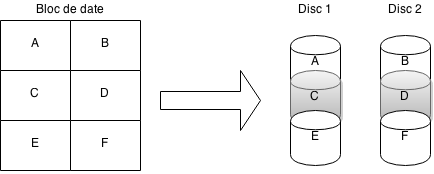
\includegraphics[width=0.6\textwidth]{img/raid0.png}
	\caption{Procesul de striping aplicat unui bloc de date}
	\label{fig:raid_strip}
	\end{center}
	\bigskip
\end{figure}

PASIS folosește schemele de partajare pentru a distribui informația nodurilor de stocare dintr-o rețea. Aceasta introduce \textit{agenți} pe partea clientului pentru a scrie sau șterge date din noduri, dar și agenți pentru mentenanță. Componentele obținute în urma partajării unui fișier sunt stocate in rețea cu ajutorul agenților (Fig. \ref{fig:pasis}). Pe lângă conținutul brut al componentelor se adaugă metadate pentru a reține adresa nodului din rețea la care au fost stocate dar și noua denumire cu care este salvată in rețea.

Atunci când un participant inițiază o cerere pentru a citi un fișier, agentul PASIS aflat local procedează dupa cum urmează:
\begin{itemize}
	\item Caută numele celor $n$ componente care alcătuiesc fișierul într-un serviciu care listează toate datele.
	\item Inițiază cereri de citire la cel puțin $k$ din cele $n$ noduri.
	\item în caz ca acesta nu primește cel puțin $k$ răspunsuri se întoarce la pasul anterior încercând interogări la noduri diferite.
	\item Reconstituie fișierul obținut din cele $k$ componente.
\end{itemize}
Operația de scriere este similară cu cea de citire, aceasta oprindu-se atunci când în cel puțin $n - k + 1$ noduri s-au stocat cu succes componente.

Autorii specifică soluții pentru auto mentenanța sistemului cu ajutorul resurselor umane prin monitorizarea periodică stării sale, folosind log-uri sau ajustarea parametrilor din cadrul schemei de partajare.

\begin{figure}
	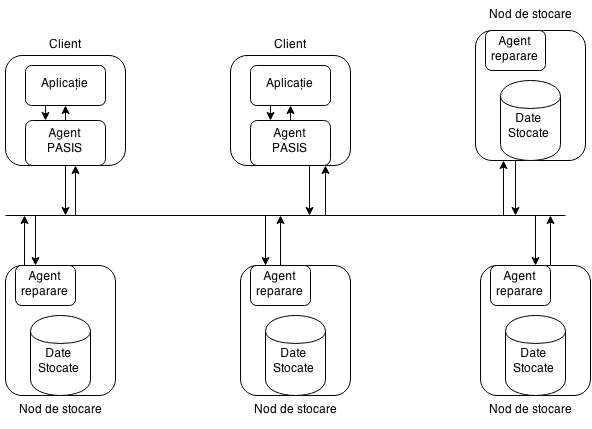
\includegraphics[width=11cm]{img/PASIS.png}
	\caption{Arhitectura PASIS cu $4$ noduri și $2$ clienți \cite{W:2000}.}
	\label{fig:pasis}
	\bigskip
\end{figure}


%------------------------------------------------------------------------------------------
%------------------------------------------------------------------------------------------
%------------------------------------------------------------------------------------------
%------------------------------------------------------------------------------------------
%------------------------------------------------------------------------------------------
%------------------------------------------------------------------------------------------

\subsection{GridSharing} 
\label{sec:desc_gridsharing}

În $2005$, Subbiah și Blough propun o nouă abordare pentru a construi un sistem de stocare securizat și tolerant la erori numit GridSharing \cite{SBM:2005}.

Subbiah și Blough folosesc un sistem care înlocuiește schemele de verificare cu o schemă de partajare unanimă XOR (considerăm cazul $q = 2$ în Fig. \ref{fig:all_or_nothing}) pentru a păstra securitatea construcției.
În cazul detectării componentelor incorecte, este adoptată o strategie de tipul replicate-and-voting.
Componentele sunt replicate pe un număr mare de servere astfel încât determinarea validității va fi stabilită în funcție de numărul de servere pe care le conțin.

Se identifică 3 tipuri de defecțiuni care pot apărea pe serverele unde sunt stocate datele:
\begin{itemize}
	\item Abandonări: un server este \textit{abandonat} dacă nu mai raspunde vreunui mesaj din rețea și s-a oprit din a mai efectua vreo operație.
	\item Bizantine: atunci când serverul nu respectă întotdeauna protocoalele inițiale iar componentele salvate local au fost compromise.
	\item Scurgeri de informații: serverul execută protocoalele corect dar e posibil ca un adversar să fi obținut componentele stocate.
\end{itemize}
Primele $2$ modele definite mai sus sunt preluate din calculul cu sisteme distribuite. Cel de-al $3$-lea model a fost introdus pentru a defini atacatorul care folosește vulnerabilitățile cu intenția de a \textit{învăța} din informații.

Arhitectura GridSharing constă în $N$ servere, unde cel mult $c$ servere pot fi abandonate, $b$ servere bizantine și $l$ cu scurgeri de informații. Cele $N$ pot fi aranjate într-un grid cu $r$ linii și $N/r$ coloane (considerăm pentru simplitate că $N \Mod r = 0$).

Caracteristicile modelului bizantin și cel specific scurgerilor de informații permit dezvăluirea componentelor unui adversar de pe cel mult $l + b$ servere.

\begin{exemplu}

	Notăm ${x \choose y}$ fiind combinări de $x$ elemente grupate câte $y$.
	Considerăm că împarțim un secret $\mathcal{S}$ la $4$ linii (participanți) astfel încât sistemul să permită $2$ componente de tip $b$, $1$ componentă de tip $l$ și $20$ servere. În cazul acesta vom folosi o schemă majoritară XOR $\big( {4 \choose 3}, {4 \choose 3}\big) = (4,4)$.

	Vom avea $4$ componente, $(s_1, s_2, s_3, s_4)$ a.î. $s_1 \oplus s_2 \oplus s_3 \oplus s_4 = \mathcal{S}$.
	Distribuirea se face in felul următor:
	\begin{itemize}
		% avem asa: p1, p2, p3, p4; s1, s2, s3
		% (p1 p2 p3, p1 p2 p4, p1 p3 p4, p2 p3 p4)
		% p1 | s4
		% p2 | s3
		% p3 | s2
		% p4 | s1
		\item Serverele situate pe prima linie primesc $s_1$
		\item Serverele situate pe a $2$-a linie primesc $s_2$
		\item Serverele situate pe a $3$-a linie primesc $s_3$
		\item Serverele situate pe a $4$-a linie primesc $s_4$
	\end{itemize}
\end{exemplu}

\begin{figure}[H]
	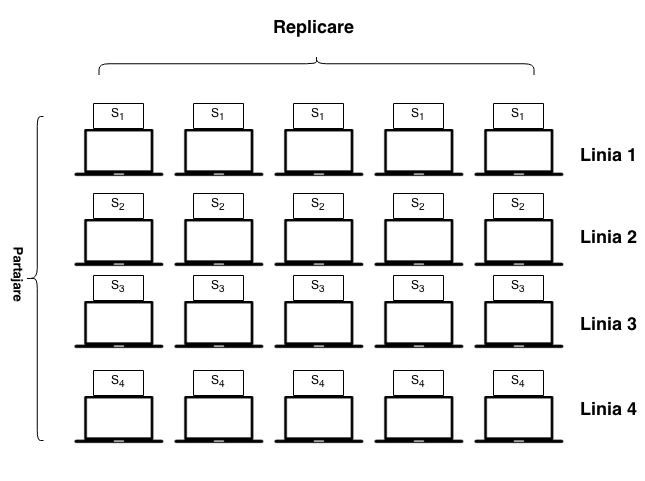
\includegraphics[width=12cm]{img/GridSharing.png}    % The printed column width is 8.4 cm.
	\caption{GridSharing cu $4$ linii, $20$ servere dintre care $2$ bizantine, $1$ cu scurgeri de informații \cite{SBM:2005}.}
	\label{fig:grid_sharing}
	\bigskip
\end{figure}


%------------------------------------------------------------------------------------------
%------------------------------------------------------------------------------------------
%------------------------------------------------------------------------------------------
%------------------------------------------------------------------------------------------
%------------------------------------------------------------------------------------------
%------------------------------------------------------------------------------------------

\subsection{POTSHARDS} 
\label{sec:desc_potshards}
în $2007$ este propus un nou sistem care combină caracteristicile PASIS și GridSharing adăugând posiblitatea de migrare a datelor la noduri noi: POTSHARDS (Protection Over Time, Securely Harboring And Reliably Distributing Stuff) \cite{SGMV:2009}.
Este de menționat faptul că autorii acestui sistem au publicat un articol în care au evidențiat vulnerabilități la numeroase sisteme de stocare (printre care și cele descrise în Secțiunile \ref{sec:desc_pasis}, \ref{sec:desc_gridsharing}) \cite{storer:2006long}.

POTSHARDS poate fi gândit ca o aplicație pe partea clientului care comunică cu o mulțime de noduri (arhive) independente, folosind reconstrucția componentelor într-un mod securizat și semnături algebrice pentru a asigura un grad ridicat de păstrare a integritații fișierelor \cite{STM:2006}.

Confidențialitatea este asigurată prin adoptarea unei scheme de partajare XOR unanimă, la fel ca în GridSharing.

Ca prim pas, POTSHARDS preprocesează fișierul într-un obiect, partajează obiectul în fragmente la care adaugă meta-date, numite \textit{shards} (Fig. \ref{fig:data-potshard}) \cite{SGMV:2009}. Acestea sunt trimise apoi arhivelor independente, fiecare având propriul domeniu de securitate, localizate in \textit{regiuni}. Pentru a reconstitui cu succes informația inițială, meta-datele shard-urilor conțin detalii despre structura pointerilor aproximativi, indicând regiunea în care se află următorul shard. Pointerii aproximativi sunt folositi pentru a reconstitui întreaga arhivă doar din shard-uri.

\begin{figure}[b!]
	\begin{center}
	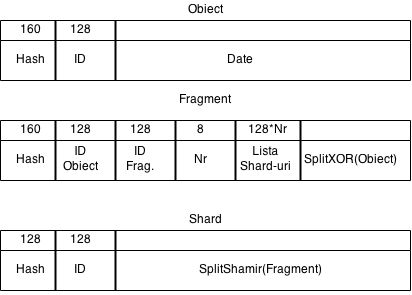
\includegraphics[width=7cm, height=4cm]{img/Shards.png}    % The printed column width is 8.4 cm.
	\caption{Entități de date in POTSHARDS. $Nr$ e numărul de shard-uri produse de un fragment.
		$SplitXOR$ reprezintă o componentă rezultată în urma partajarii unanime XOR. Analog $SplitShamir$ reprezintă o componentă rezultată în urma partăjarii folosind schema Shamir \cite{SGMV:2009}}
	\label{fig:data-potshard}
	\bigskip
	\end{center}
\end{figure}

Procesul de fragmentare a datelor este prezentat in Fig. \ref{fig:potshards-layers}.


\begin{figure}
	\begin{center}
	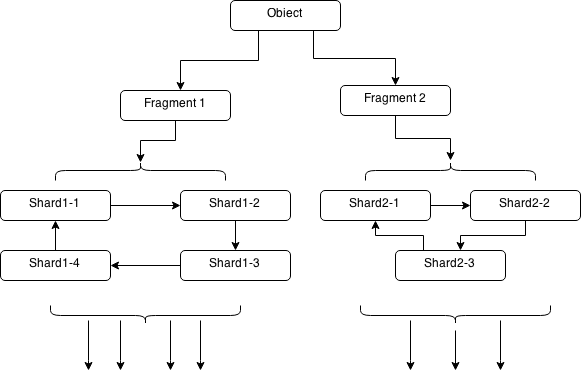
\includegraphics[width=12cm]{img/POTSHARDS.png}    % The printed column width is 8.4 cm.
	\caption{Distribuirea unui obiect in POTSHARDS}
	\label{fig:potshards-layers}
	\bigskip
	\end{center}
\end{figure}

Pentru ca reconstituirea unui fișier sa fie fezabilă unui utilizator, acestuia îi este întoarsă o listă cu locațiile exacte shard-urilor corespunzătoare.
Obținerea unui shard de către un atacator nu este fezabilă, pentru a detecta următorul shard, un atac brut force constă în cereri multiple în zona indicată de pointerul aproximativ. Un astfel de atac nu va trece neobservat de POTSHARDS deorece unul dintre scopurile sale este să stocheze datele distribuite într-un mod cât mai uniform \cite{SGMV:2009}.


%------------------------------------------------------------------------------------------
%------------------------------------------------------------------------------------------
%------------------------------------------------------------------------------------------
%------------------------------------------------------------------------------------------
%------------------------------------------------------------------------------------------
%------------------------------------------------------------------------------------------

\section{Sistemul de stocare Alouneh et al. (2013)}
\label{sec:desc_alouneh}

Alouneh et al. propun un sistem pentru stocarea sigură a datelor un timp indelungat folosind schema Shamir cu câteva modificări. Aceste schimbări se vor arăta esențiale mai târziu în menținerea securității \cite{AAMK:2013}.

Pentru stocarea unui fișier în sistem (abordând filozofia majorității sistemelor de operare - orice este un fișier), o aplicație client îl împarte în blocuri de octeți de lungime $k$. Pentru fiecare bloc, octeții devin coeficienții unui polinom $f$ de grad $k$, componenta corespunzătoare participantului $i$ va fi reprezentată de valoarea lui $f(i)$, $i = \{1,2,\dots, n\}$. 
Menționăm că toate operațiile se vor efectua in $GF(256)$ modulo un polinom ireductibil (în implementarea sistemului, autorii folosesc $x^8 + x^5 + x^3 + x + 1$). Procedeul este descris in detaliu in Fig \ref{fig:alouneh_distribution}.


%---------------- Figure - alouneh-distribution - START ------------------------
\begin{figure*}[h!]

\begin{tabular}{|p{\textwidth}|}
\hline

\\
\hspace{.1in}
\textbf{Date de intrare}: Un fișier binar $\mathcal{S}$;
\medskip

\hspace{.1in}
\textbf{Date de ieșire}: $n$ fișiere binare distribuite la noduri din rețea;
\medskip

\hspace{.1in}
\textbf{Procesarea componentelor}: Aplicația existentă pe partea clientului: 
	\begin{itemize}
		\item Dacă $\mathcal{S}$ nu are o lungime divizibilă cu $k$:
			\begin{itemize}
			\item Concatenează la sfârsitul lui $\mathcal{S}$ octeți până când $len(\mathcal{S}) \Mod k = 0$;
			\end{itemize}
		\item Împarte $\mathcal{S}$ în blocuri de lungime $k$;
		\item Repetă pentru fiecare bloc $B_t$ de lungime $k$:
		\begin{itemize}
			\item Construiește polinomul $f(x) = B_{t_{k - 1}}x ^ {k-1} + B_{t_{k - 2}}x ^ {k - 2} + .... + B_{t_1}x + B_{t_0}$;
			\item Calculează $f(i)$ pentru $1 \leq i \leq n$;
		\end{itemize}
	\end{itemize}

\hspace{.1in}
\textbf{Distribuție}: Aplicația la nivelul clientului:
	\begin{itemize}
		\item Distribuie componenta $f(i)$ nodului din rețea cu indicele $i$:
	\end{itemize}

\\
\hline
\end{tabular}
\caption{Schema Alouneh et al. - Generare \cite{AAMK:2013}}
\label{fig:alouneh_distribution}
\end{figure*}

%---------------- Figure - alouneh_distribution - STOP ------------------------

\begin{exemplu}
Vom exemplifica modul de calcul în $GF(256) \Mod {g(x)} $ unde $g(x) = x ^ 8 + x ^ 4 + x ^ 3 + 1$. Luăm polinomul $f(x) = 10 + 15x$ corespunzător unui fișier format din octeții (în această ordine) $10$ $15$.
	\begin{equation} \label{eq:f_01}
	\begin{split}
		f(01) \Mod{g(x)} & = 10 + 15 \Mod{g(x)} \\
		& = (x ^ 4) + (x ^ 4 + x ^ 2 + 1) \Mod{g(x)} \\
		& = x ^ 2 + 1 = 000000101_{(2)} \\
		& =  05_{(16)}
	\end{split}
	\end{equation}

	\begin{equation} \label{eq:f_02}
	\begin{split}
	 f(02) \Mod{g(x)} & = 10 + 15\cdot02 \Mod{g(x)} \\
	 & = (x ^ 4) + (x ^ 5 + x ^ 3 + x) \Mod{g(x)} \\
	 & = 00111010_{(2)} \\
	 & = 3A_{(16)}
	 \end{split}
	 \end{equation}
\end{exemplu}
Reconstituirea unui fișier (Fig. \ref{fig:alouneh_reconstruction}) se realizează din orice mulțime de componente $A$ de dimensiune minim $k$ folosind interpolarea Lagrange (utilizată și în cadrul schemei Shamir):
\begin{equation}
	\label{eq:lagrange_poly}
	f(x)=\sum_{i \in A} f(i) \prod_{j \in A, j \neq i} \frac{x-j}{i-j}
\end{equation}

\begin{exemplu}
Vom exemplifica interpolarea conform ecuației {\ref{eq:lagrange_poly}} folosind componentele (\ref{eq:f_01}) și (\ref{eq:f_02}) calculate în exemplul anterior:
	\begin{equation}
	\begin{split}
		f(x) & = 05(x - 02)(01 - 02)^{-1} + 3A(x - 01)(02 - 01)^{-1} \\
		& = 05(x - 02)03^{-1} + 3A(x - 01)03^{-1} \\
		& = F6(05 + 3A)x + F6(05\cdot02 + 3A \cdot 01) \\
		& = F6\cdot 3F\cdot x + F6\cdot30 = 15x + 10
	\end{split}
	\end{equation}
\end{exemplu}

Noutatea arhitecturii constă in diminuarea redundanței componentelor la un factor de $k$, spre deosebire de sistemele descrise in Secțiunile \ref{sec:desc_pasis}, \ref{sec:desc_gridsharing} și \ref{sec:desc_potshards}. Reducerea spațiului ocupat de componente este datorat înlocuirii coeficienților generați aleator din schema Shamir cu octeții din fișierul ce va fi partajat, fiecare componentă având nevoie de $1/k$ din dimensiunea fișierului $\mathcal{S}$.

Abordarea acestei metode deterministe conduce la insecuritatea sistemului, Alouneh et al. afirmând în mod eronat că securitatea este indusă în mod automat de schema Shamir. 

%---------------- Figure - alouneh-reconstruction- START ------------------------
\begin{figure*}[h!]

\begin{tabular}{|p{\textwidth}|}
\hline

\\
\hspace{.1in}
\textbf{Date de intrare}: Cel puțin $k$ componente provenite din noduri (distincte);
\medskip

\hspace{.1in}
\textbf{Date de ieșire}: Fișierul binar original $\mathcal{S}$;
\medskip

\hspace{.1in}
\textbf{Reconstrucție}: Aplicația existenta pe partea clientului: 
	\begin{itemize}
		\item Repetă pentru fiecare bloc al lui $\mathcal{S}$:
		\begin{itemize}
			\item Calculează prin interpolare coeficienții lui $f(x)=B_{t_{k - 1}}x ^ {k-1} + B_{t_{k - 2}}x ^ {k - 2} + .... + B_{t_1} + B_{t_0}$
			\item Reconstituie blocul $B_t$
		\end{itemize}
		\item șterge octeții de la sfârșitul fișierului adăugați la generare. 
	\end{itemize}

\\
\hline
\end{tabular}
\caption{Schema Alouneh et al. - Reconstrucție \cite{AAMK:2013}}
\label{fig:alouneh_reconstruction}
\end{figure*}

%---------------- Figure - alouneh_reconstruction- STOP ------------------------



%------------------------------------------------------------------------------------------
%------------------------------------------------------------------------------------------
%------------------------------------------------------------------------------------------
%------------------------------------------------------------------------------------------
%------------------------------------------------------------------------------------------
%------------------------------------------------------------------------------------------

\section{Contribuții}
\label{sec:alouneh_contributions}

În \cite{RD:2015} am analizat sistemul Alouneh et al. prezentat în Secțiunea \ref{sec:desc_alouneh}. Am indentificat erori majore ale acestuia și am implementat sistemul descris de autori pentru a demonstra practic, nu doar teoretic, anumite greșeli pe care le vom evidenția în următoarele secțiuni.

\subsection{Vulnerabilități evidențiate}

Spre deosebire de schema Shamir, unde coeficienții (cu excepția termenului liber, care este egal cu secretul) sunt aleși într-un mod aleator uniform, sistemul propus de Alouneh et al. folosește o schemă modificată Shamir în care coeficienții sunt extrași din conținutul fișierelor originale.
Alegerea este motivată de faptul ca mulțimea componentelor și efortul computațional depus pentru generarea coeficienților se reduce la un factor de $k$ ori, spre deosebire de schema Shamir.

Datorită determinismului, partajarea unui fișier de mai multe ori implică obținerea de componente identice.
Determinismul duce la câteva atacuri simple în momentul în care un atacator obține informațiile stocate într-un nod, indiferent de mărimea pragului folosit în metoda de partajare. În acest sens, am evidențiat $2$ atacuri simple în cazul în care componentele sunt calculate in ordine ($f(01), f(02), \dots$):
\begin{itemize}
	\item Detectarea tipului unui fișier
	\item Detectarea conținutului unui fișier
\end{itemize}

Deoarece Alouneh et al. nu menționeaă o metodă de padding, am indicat că un atac bazat pe felul în care se realizează completarea fișierului (padding) $\mathcal{S}$, înainte de partajarea sa poate fi fezabil, în condițiile în care s-a demonstrat că această alegere este esențială în păstrarea securității \cite{Vaudenay:2002}.

\subsubsection{Detectarea tipului de fișier}\hspace*{\fill} \\
\label{subsec:file_type_detection}

În tehnologia informației, la inceputul fiecărui fișier se află o secvență de octeți (denumită semnătură sau antet) cu rolul de a identifica tipul acestuia. Tabelul {\ref{table:sign}} indică $7$ din cele mai uzuale antete.


%-----------------------------------------------------
\begin{table}[b]
\bigskip
\begin{center}
\caption{Semnături de fișiere}\label{tb:margins}
\label{table:sign}
\begin{tabular}{ccccc}
Tip de fișier &  \multicolumn{4}{c}{Primii 4 octeți}\\ \hline 
doc &  D0 & CF & 11 & E0\\
gif & 47 & 49 & 46 & 38 \\
pdf & 25 & 50 & 44 & 46 \\
png & 89 & 50 & 4E & 47 \\
rar & 52 & 61 & 72 & 21 \\
wav & 52 & 49 & 46 & 46 \\
zip & 50 & 4B & 03 & 04\\  \hline
\end{tabular}
\end{center}
\bigskip
\end{table}

Se consideră cazul în care partajarea unui fișier \textit{pdf} se face cu ajutorul sistemului descris in {S}ecțiunea \ref{sec:desc_alouneh}, folosind $k \leq 4$. Polinomul corespunzător $f(x)$ va fi intotdeauna același. Presupunând ca numerotarea nodului $i$ este aceeași, putem determina cu ușurință dacă este stocat un fișier \textit{pdf} fără a lua în calcul conținutul fișierului.
Acest atac este fezabil deorece valoarea lui $k$ este publică iar $i$ poate să fie descoperit în momentul distribuirii.

Cu alte cuvinte, dacă un adversar obt\c{i}ne controlul unui singur nod, bazându-se doar pe valoarea primei componente poate detecta tipul unui fișier.

Pentru a exemplifica, un adversar poate distinge cu probabilitate ridicată între fișierele \textit{doc, gif, pdf, png, rar, wav} și \textit{zip}. În Tabelul {\ref{table:shares}} avem generate componentele pentru $k = 2$ și $n = 5$.
Dacă un adversar descoperă valoarea primului nod iar prima componentă este $14$ atunci acesta știe cu certitudine că aceasta corespunde un fișier \textit{gif}. Dacă obține accesul nodului $4$ și citește valoarea $205$ atunci știe că fișierul este de tipul \textit{rar}. Daca citește valoarea $27$ de pe primul nod atunci știe că poate fi un \textit{wav} sau \textit{zip}; apoi poate să distingă cele 2 fișiere cu probabilitate $1$ dacă dezvăluie o singură valoare de pe celelalte noduri ($2$, $3$, $4$ sau $5$) pentru că valorile sunt distincte.


%-----------------------------------------------------
\begin{table}[t]
\begin{center}
\caption{Componentele primului bloc ($k=2$)}\label{tb:margins}
\label{table:shares}
\begin{tabular}{cccccccc}
Tip fișier & Nod 1 & Nod 2 & Nod 3 & Nod 4 & Nod 5 \\
  & ($i=1$) & ($i=2$) & ($i=3$) & ($i=4$) & ($i=5$) \\
\hline
doc & 31 & 85 & 154 & 193 & 14 \\
gif & 14 & 213 & 156 & 120 & 49 \\
pdf & 117 & 133 & 213 & 126 & 46 \\
png & 217 & 41 & 121 & 210 & 130 \\ 
rar & 51 & 144 & 241 & 205 & 172  \\
wav & 27 & 192 & 137 & 109 & 36 \\
zip & 27 & 198 & 141 & 103 & 44 \\ \hline
\end{tabular}
\end{center}
\bigskip
\end{table}


%------------------------------------------------------------------------------------------
%------------------------------------------------------------------------------------------


\subsubsection{Detectarea de conținut}\hspace*{\fill} \\
\label{subsec:file_content_detection}

Multe documente urmează un anumit tipar precum contracte, chitanțe, bonuri fiscale sau curriculum vitae. Deoarece majoritatea conținutului rămâne neschimbat, există o probabilitate destul de mare ca multe componente sa aibă aceeași valoare. O dată ce un adversar reușește să determine componentele unui nod, poate determina prin analogie tipul de conținut al fișierului original.

Fișierele vulnerabile sunt cele care conțin o secvență de octeți periodică (imagini cu un pattern repetitiv) sau cele care au preponderent octeți nuli (valoarea componentelor asociată majorității blocurilor fiind $0$). Spre deosebire de prima metodă, aceasta nu necesită compararea cu un al $2$-lea fișier, tratând componentele de sine stătător. Multiple componente identice indică existența unor secvențe repetitive în conținutul fișierului.


%------------------------------------------------------------------------------------------
%------------------------------------------------------------------------------------------

\subsection{Implementare și rezultate practice}
Pentru a arăta aplicabilitatea rezultatelor în practică, am implementat propunerea descrisa in Secțiunea {\ref{sec:desc_alouneh}} și am testat pe câteva cazuri.

În cadrul implementării am folosit limbajul Python 3.0 sub sistemul de operare ArchLinux. Python este un limbaj high-level, permițând programatorilor să exprime concepte în mai puține linii de cod față de C++ sau Java și este disponibil sub licență open-source \cite{Python:2015}.
Pentru a realiza comunicarea între procese am folosit Cerealizer iar distribuția componentelor a fost generată grafic cu ajutorul pachetului Matplotlib \cite{Hunter:2007, PyCerealizer:2015}. De asemenea am folosit sistemul de versionare Git iar în prezent codul folosit este găzduit de GitHub \cite{Github:2015, CodeGit:2015}.

Având în vedere că articolul original nu menționează o metodă de padding, am considerat o metodă standard pentru a completa octeții ultimului bloc: alipim la sfârșitul lui $\mathcal{S}$ octeții $80$ $00$ $\dots$ $00$ $00$ până când lungimea ultimului bloc ajunge la $k$ octeți.

Menționăm această metodă doar pentru completitudine, aceasta neafectând rezultatele, care consideră doar secvențele de octeți din antet sau de la începutul fișierului.


%------------------------------------------------------------------------------------------
%------------------------------------------------------------------------------------------

\subsubsection{Detectarea tipului de fișier}\hspace*{\fill} \\

Extindem analiza făcută în Secțiunea {\ref{subsec:file_type_detection}} asupra tipurilor de fișiere din Tabelul {\ref{table:sign}} pentru $k = 2$ și creștem valoarea indicelui $i$ până când 2 componente devin egale. Fie $f_l$ polinomul de gradul $1$ asociat primului bloc al fișierului aflat pe linia $l$. Analog $f_c$ polinomul de gradul $1$ asociat primului bloc al fișierului aflat pe coloana $c$.

Tabelul {\ref{table:k2} prezintă} valoarea maximă a nodul $i$ pentru care $f_l(i) \neq f_c(i)$. Valoarea $-1$ indică lipsă de coliziuni ale lui $f_c(x)$, $f_l(x)$ pentru $i$, $i = {1,2,\dots,255}$ ($\not\exists 1 \leq i \leq 255$ a.î. $f_l(i) = f_c(i)$)).

Deoarece pe diagonala principală toate componentele sunt identice pentru $k \leq 4$, poate fi ignorată. în Tabelul {\ref{table:k2}} observăm valoarea $0$ pentru perechea $(wav, zip)$ pentru că $f_{wav}(1) = f_{zip}(1) = 27$ (Tabelul \ref{table:sign}).



%-----------------------------------------------------
\begin{table}[b]
\begin{center}
\caption{Indicele maxim $i$ a.î. componentele primului bloc sa fie distincte($k=2$)}\label{tb:margins}
\label{table:k2}
\begin{tabular}{cccccccc}
Tip Fișier & doc & gif & pdf & png & rar & wav & zip \\\hline
  doc & - & 169 & 194 & 209 & 170 & 206 & 110\\
  gif & 169 & - & 133 & 137 & 75 & -1 & 133\\
  pdf & 194 & 133 & - & -1 & 115 & 151 & 133\\
  png & 209 & 137 & -1 & - & 229 & 147 & 195\\
  rar & 170 & 75 & 115 & 229 & - & -1 & 42\\
  wav & 206 & -1 & 151 & 147 & -1 & - & 0\\
  zip & 110 & 133 & 133 & 195 & 42 & 0 & -\\ \hline
\end{tabular}
\end{center}
\end{table}

Tabelele {\ref{table:k3} și \ref{table:k4}} prezintă rezultatele pentru $k = 3$ și $k = 4$. Pentru $k \geq 5$ este nevoie de un antet cu mai mult de $4$ octeți.

Considerăm metoda de distribuire descrisă exact ca în Tabelul {\ref{fig:alouneh_distribution}}, și anume nodul de stocare $i$ primește componenta $f(i)$.
Dacă un atacator preia controlul nodului cu valoarea $i$, acesta poate face distincția între tipul a $2$ fișiere partajate cu probabilitate $1$ dacă $i$ e mai mic decât valoarea afișată în tabel.

Spre exemplu, un adversar care obține accesul unui singur nod de stocare, iar partajarea a fost făcută pentru $k=2$ poate distinge cu probabilitate $1$ între un fișier $doc$ sau $pdf$ dacă $i \leq 194$. Deoarece $n > 194$ nu se întâmplă în practică, acest atac funcționează. Faptul că multe valori sunt ridicate și majoritatea sunt $-1$ (Tabelul \ref{table:k3}), indică un nivel scăzut de securitate al schemei. În cazul celor cu $-1$ un adversar va câștiga întotdeauna cu probabilitatea $1$, indiferent de indicele nodului de stocare pe care îl obține.

Precizăm că acest atac funcționează doar dacă nodurile de stocare își păstrează indexul în cazul partajării repetate a.î. aplicația disponibilă pe partea de client calculează cele $n$ valori $f(i_1),\dots,f(i_2)$ pentru $i_1,\dots,i_n$ distincte și păstrează nodul $j$ asociat lui $i_j$.


%------------------------------------------------------------------------------------------
%------------------------------------------------------------------------------------------
\begin{table}[t]
\begin{center}
\caption{Indicele maxim $i$ a.î. componentele primului bloc sa fie distincte($k=3$)}\label{tb:margins}
\label{table:k3}
\begin{tabular}{cccccccc}
Tip Fișier & doc & gif & pdf & png & rar & wav & zip \\\hline
  doc & - & 63 & -1 & -1 & -1 & -1 & -1\\
  gif & 63 & - & -1 & -1 & -1 & -1 & -1\\
  pdf & -1 & -1 & - & 164 & -1 & 119 & -1\\
  png & -1 & -1 & 164 & - & 143 & 122 & 129\\
  rar & -1 & -1 & -1 & 143 & - & 143 & -1\\
  wav & -1 & -1 & 119 & 122 & 143 & - & 172\\
  zip & -1 & -1 & -1 & 129 & -1 & 172 & -\\ \hline
\end{tabular}
\end{center}
\bigskip
\end{table}

%-----------------------------------------------------
\begin{table}[t]
\begin{center}
\caption{Indicele maxim $i$ a.î. componentele primului bloc sa fie distincte($k=4$)}\label{tb:margins}
\label{table:k4}
\begin{tabular}{cccccccc}
Tip Fișier & doc & gif & pdf & png & rar & wav & zip \\\hline
  doc & - & -1 & 38 & 95 & 1 & 95 & 98\\
  gif & -1 & - & -1 & -1 & 167 & -1 & -1\\
  pdf & 38 & -1 & - & 12 & 11 & 119 & 70\\
  png & 95 & -1 & 12 & - & 243 & 95 & 148\\
  rar & 1 & 167 & 11 & 243 & - & -1 & 94\\
  wav & 95 & -1 & 119 & 95 & -1 & - & -1\\
  zip & 98 & -1 & 70 & 148 & 94 & -1 & -\\ \hline
\end{tabular}
\end{center}
\bigskip
\end{table}

\subsubsection{Detectarea de conținut} \hspace*{\fill} \\

Considerăm scenariul pentru detectarea conținutului unui fișier, demonstrând practic cum un adversar poate să facă diferența între $2$ componente stocate pe același nod aparțin unor documente similare. Atacul presupune accesul la un singur nod, indiferent de mărimea pragului $k$.


Pentru experiment am ales $3$ fișiere \textit{pdf} disponibile online la {\cite{Europass:2015}}:
\begin{itemize}
  \item Europass Curriculum Vitae - BG, Bulgaria;
  \item Europass Curriculum Vitae - DK, Dannemark;
  \item Europass Mobility - RO, Romania.
\end{itemize}

%-----------------------------------------------------

\begin{figure}[b!]
\begin{center}{}
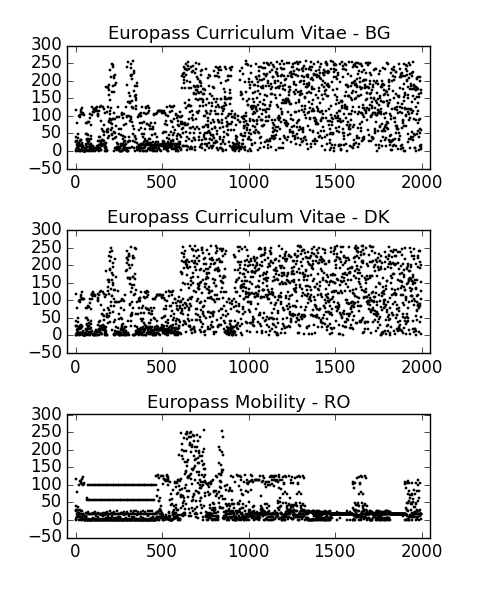
\includegraphics[width=0.53\textwidth]{img/db1.png}    % The printed column width is 8.4 cm.
\caption{Nod 1: Graficul componentelor pentru primele 2000 de blocuri} 
\label{fig:db1}
\end{center}
\end{figure}

%-----------------------------------------------------


%-----------------------------------------------------
\begin{figure}[t!]
\begin{center}
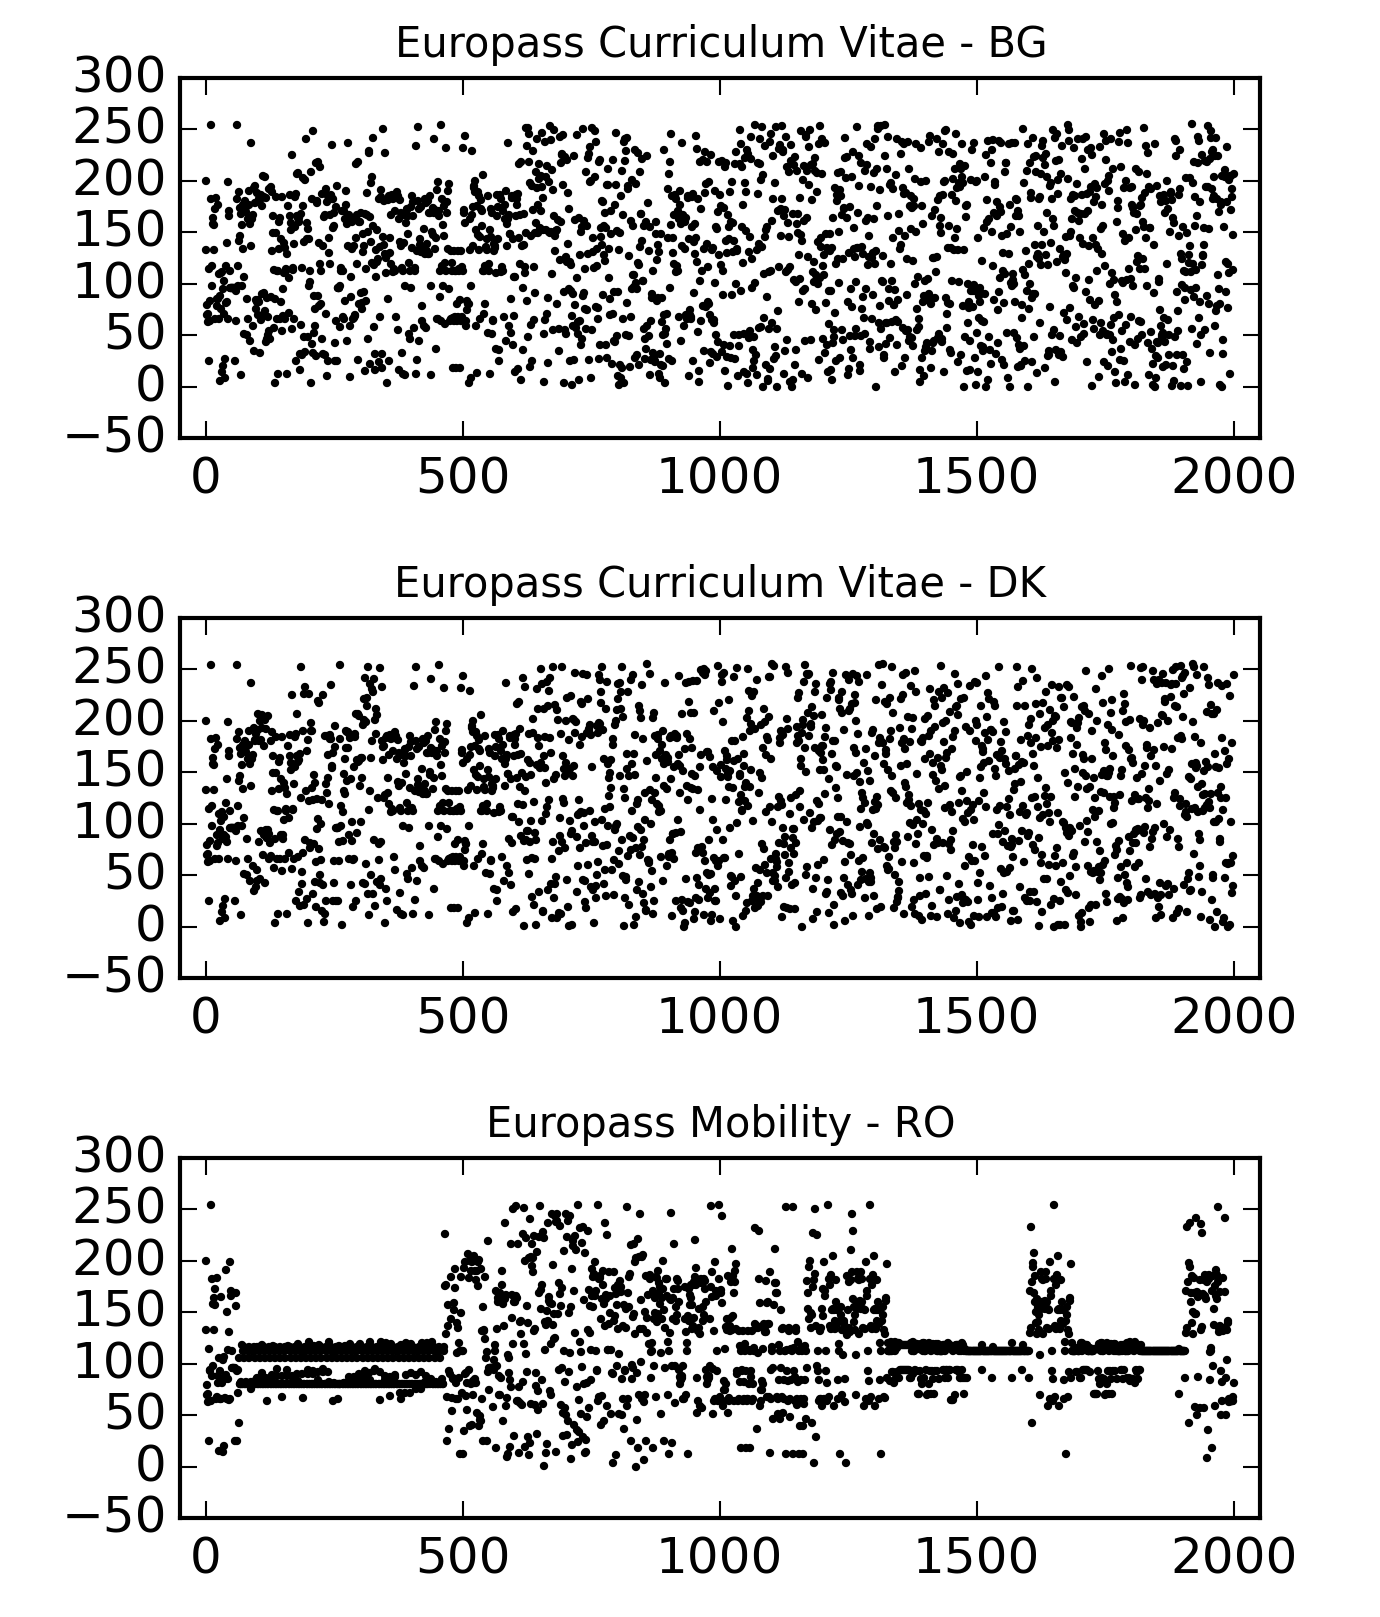
\includegraphics[width=0.53\textwidth]{img/db2.png}    % The printed column width is 8.4 cm.
\caption{Nod 2: Graficul componentelor pentru primele 2000 de blocuri} 
\label{fig:db2}
\end{center}
\end{figure}
%-----------------------------------------------------

%-----------------------------------------------------
\begin{figure}[b!]
\begin{center}
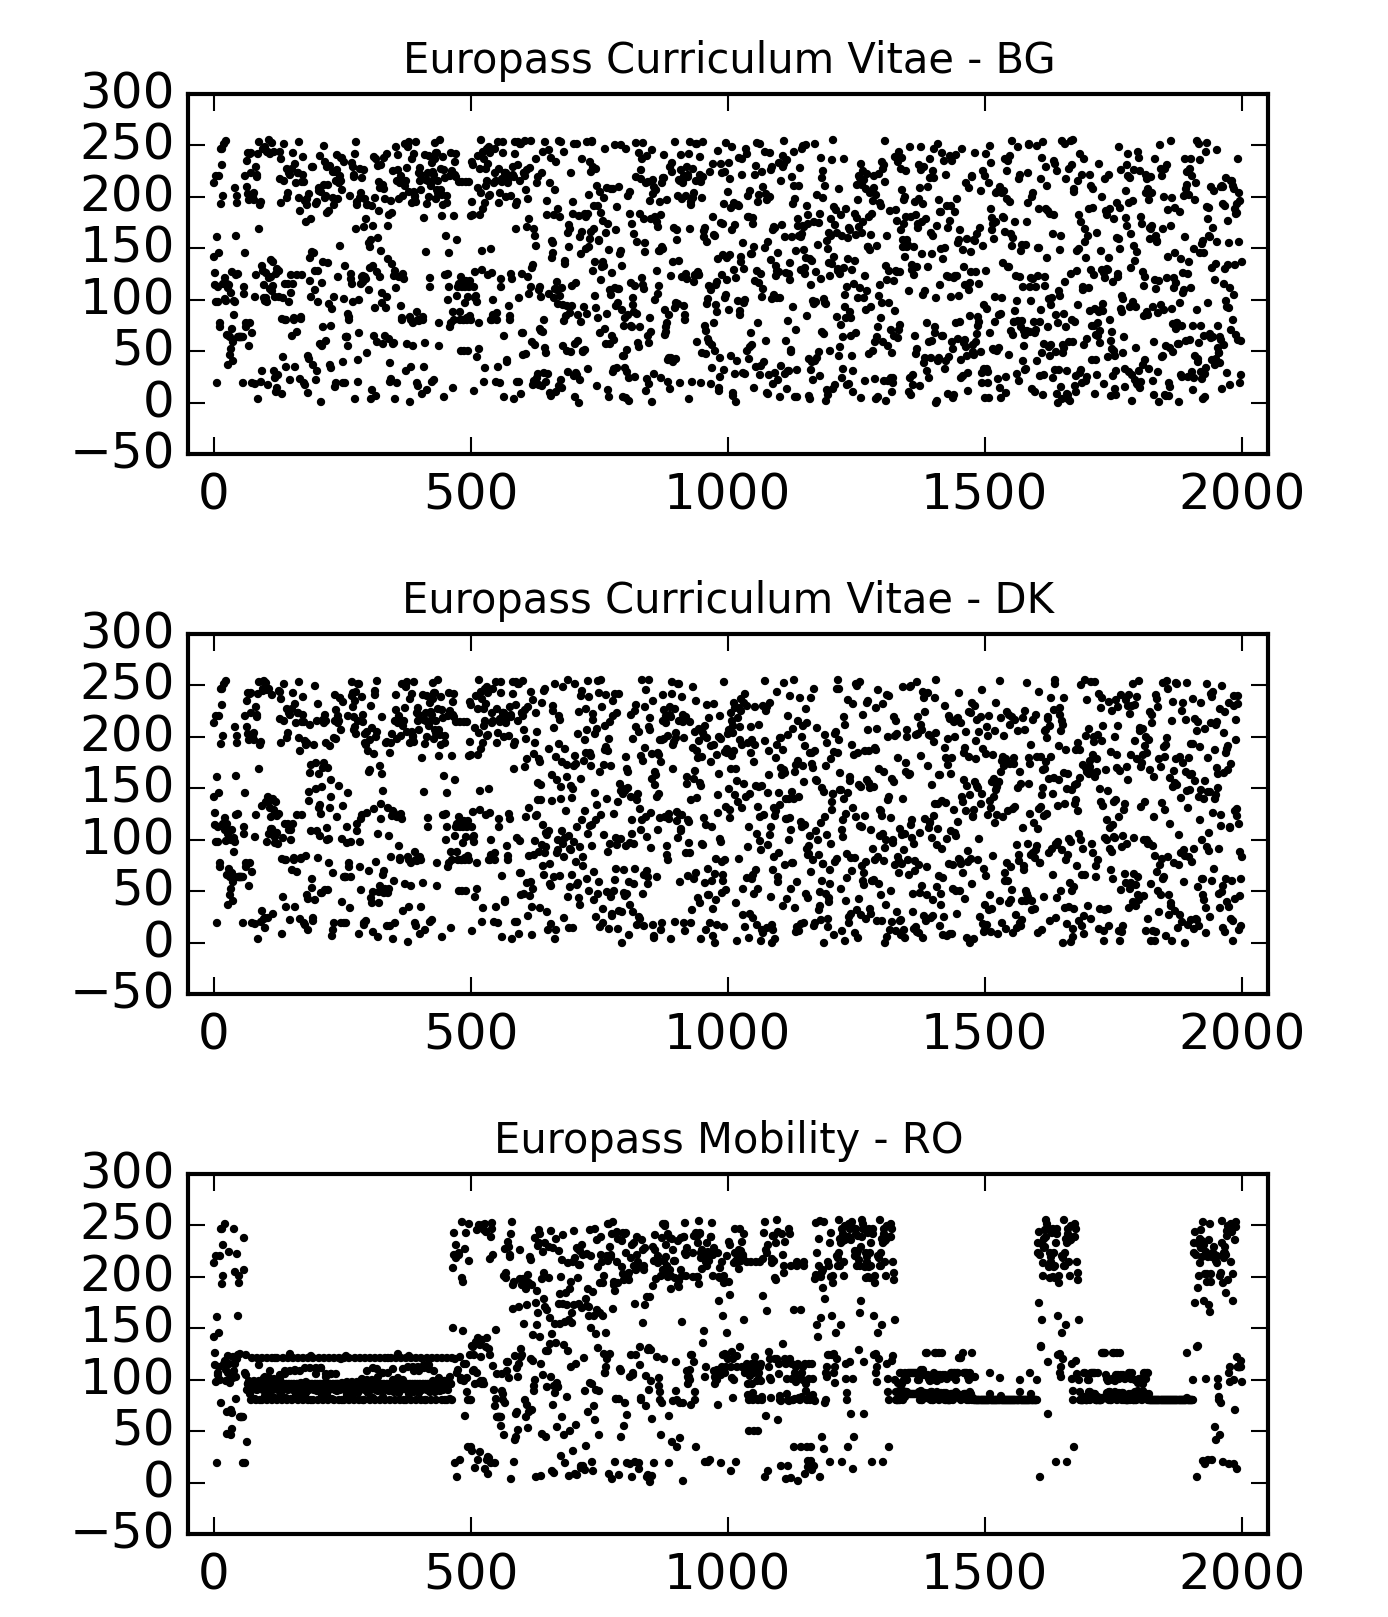
\includegraphics[width=0.53\textwidth]{img/db3.png}    % The printed column width is 8.4 cm.
\caption{Nod 3: Graficul componentelor pentru primele 2000 de blocuri} 
\label{fig:db3}
\end{center}
\end{figure}
%-----------------------------------------------------

%----------------------------------------------------
\begin{figure}[t!]
\begin{center}
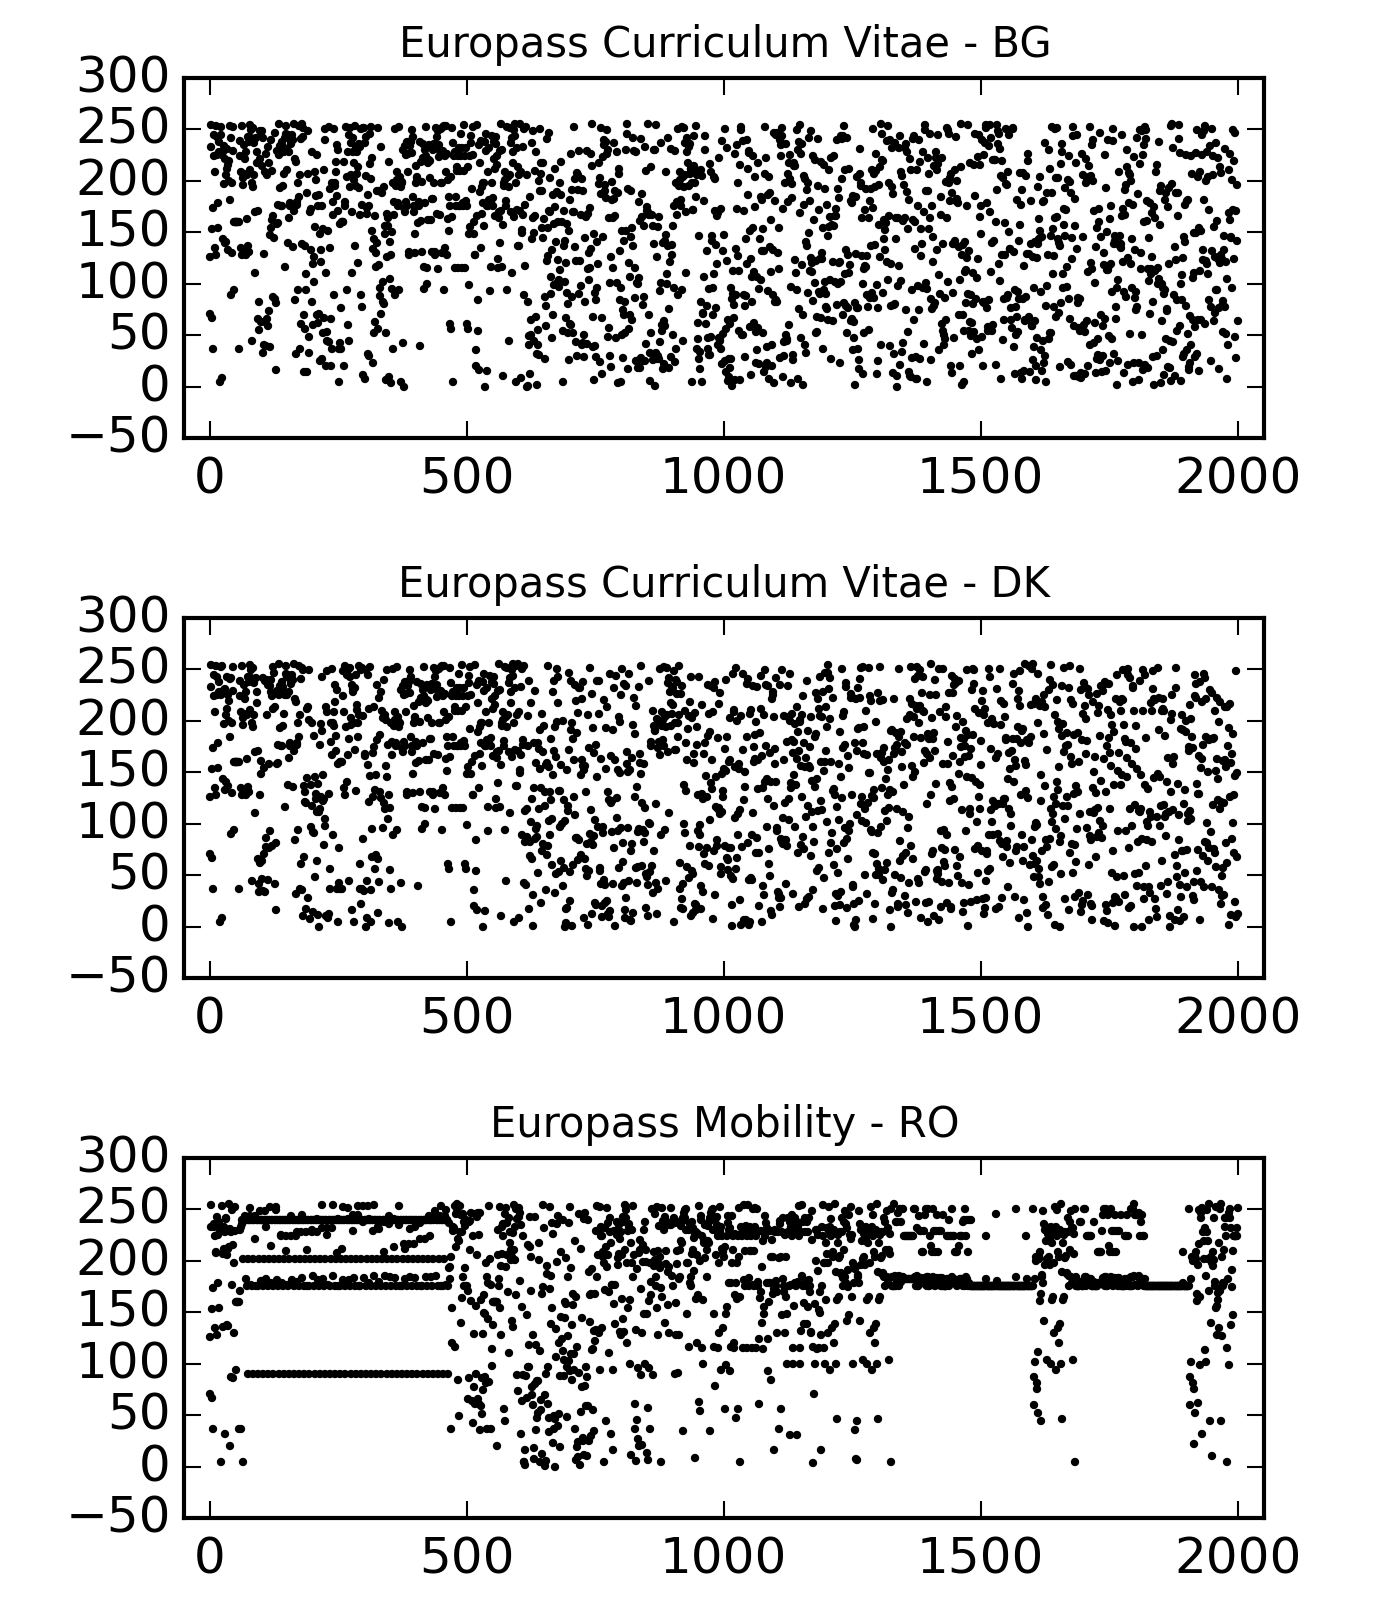
\includegraphics[width=0.53\textwidth]{img/db4.png}    % The printed column width is od8.4 cm.
\caption{Nod 4: Graficul componentelor pentru primele 2000 de blocuri} 
\label{fig:db4}
\end{center}
\end{figure}
%-----------------------------------------------------
%-----------------------------------------------------




Primele două fișiere reprezintă șablonul pentru un CV european în limba bulgară, respectiv daneză. Observăm că nu doar conținutul șabloanelor diferă, dar și limba în care au fost traduse. Cel de-al treilea fișier este complet diferit de primele două, fiind un document personal în limba română, folosit pentru înregistrarea cunoștiintelor dobăndite într-o țară europeană.

Pentru a arăta vulnerabilitatea sistemului Alouneh et al. {\cite{AAMK:2013}}, partajăm cele $3$ fișiere folosind schema $(2, 4)$. Experimentul reprezintă o implementare practică a metodei prezentate in Fig. {\ref{fig:alouneh_distribution}}.

Fig. {\ref{fig:db1}}, {\ref{fig:db2}}, {\ref{fig:db3}}, {\ref{fig:db4}} conțin $2000$ de componente generate pentru cele $3$ fișiere, stocate în baza de date corespunzătoare nodurilor $1,2,3$ și $4$. Presupunem că indicele $i$ este fixat, polinoamele fiind evaluate în același nod $i$. Un adversar care obține componentele unui nod poate deduce cu ușurintă graficul lor.

Considerăm că un adversar reușește să obțină componentele din Fig. {\ref{fig:db1}}. Poate deduce ușor că primele două fișiere au un număr mare de componente identice iar cel de-al $3$-lea este diferit de primele.

Din cauza șablonului pe care îl respectă cele două CV-uri, un adversar are nevoie în cazul de față doar de primele $500$ de componente pentru a constata similiaritatea celor $2$ cu o probabilitate ridicată.
Diferența vizuala este evidentă între oricare din cele $4$ grafice, deci un adversar poate reuși să afle informații despre fișierele partajate indiferent de nodul de stocare vulnerabil.

Considerăm în continuare un alt scenariu, în care partajăm o imagine pentru care informația se repetă. Fie imaginea din Fig. {\ref{fig:carouri}} partajată folosind schema din Secțiunea {\ref{sec:desc_alouneh}}, având $4$ noduri iar informația stocată pe cel puțin $2$ din ele pot reconstitui imaginea partajată inițial. {\ref{fig:alouneh_distribution}}. La fel ca în exemplul precedent, Fig. {\ref{fig:carouri_db1}, \ref{fig:carouri_db2}, \ref{fig:carouri_db3}, \ref{fig:carouri_db4}} reprezintă grafic componentele imaginii din Fig. {\ref{fig:carouri}}. Un adversar constată cu ușurință prin obținerea informațiilor stocate aflate pe un singur nod (indiferent de mărimea pragului $k$) că fișierul original conține un pattern care se repetă.


%-----------------------------------------------------
\begin{figure}[H]
\begin{center}

\includegraphics[width=0.35\textwidth]{img/carouri.png}    % The printed column width is 8.4 cm.
\caption{Imagine conținând pattern-uri} 
\label{fig:carouri}
\end{center}
\end{figure}
%-----------------------------------------------------


%-----------------------------------------------------
\begin{figure}[t!]
\begin{center}
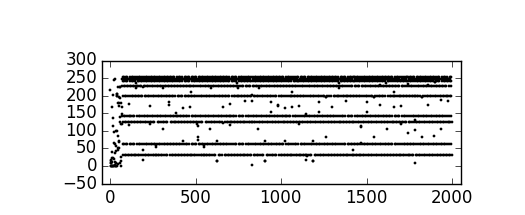
\includegraphics[width=0.55\textwidth]{img/carouri_db1.png}    % The printed column width is 8.4 cm.
\caption{Nod 1: Graficul componentelor pentru primele 2000 de blocuri} 
\label{fig:carouri_db1}
\end{center}
\end{figure}
%-----------------------------------------------------

%-----------------------------------------------------
\begin{figure}[t!]
\begin{center}
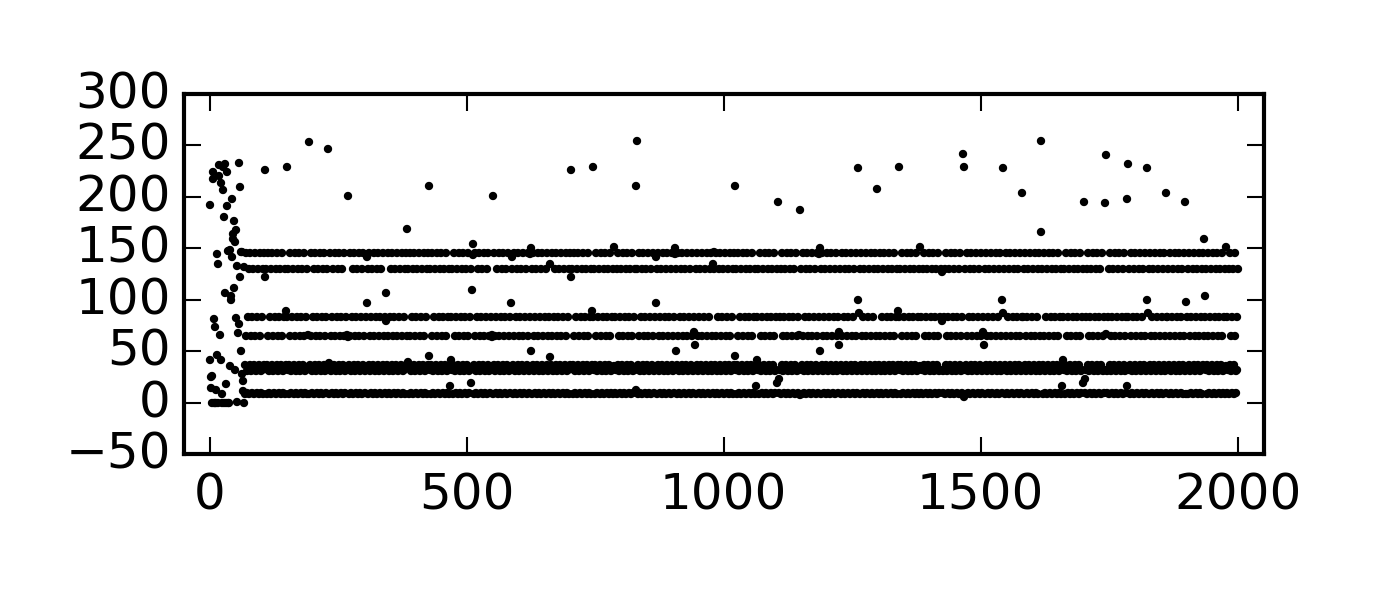
\includegraphics[width=0.55\textwidth]{img/carouri_db2.png}    % The printed column width is 8.4 cm.
\caption{Nod 2: Graficul componentelor pentru primele 2000 de blocuri} 
\label{fig:carouri_db2}
\end{center}
\end{figure}
%-----------------------------------------------------

%-----------------------------------------------------
\begin{figure}[t!]
\begin{center}
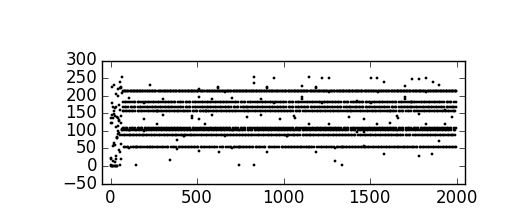
\includegraphics[width=0.55\textwidth]{img/carouri_db3.png}    % The printed column width is 8.4 cm.
\caption{Nod 3: Graficul componentelor pentru primele 2000 de blocuri} 
\label{fig:carouri_db3}
\end{center}
\end{figure}
%-----------------------------------------------------

%-----------------------------------------------------
\begin{figure}[t!]
\begin{center}
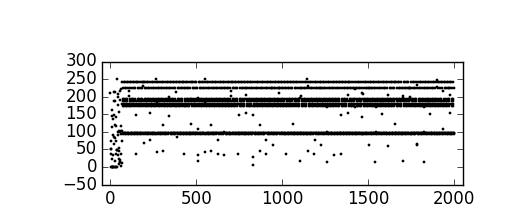
\includegraphics[width=0.55\textwidth]{img/carouri_db4.png}    % The printed column width is 8.4 cm.
\caption{Nod 4: Graficul componentelor pentru primele 2000 de blocuri} 
\label{fig:carouri_db4}
\end{center}
\end{figure}
%-----------------------------------------------------


%------------------------------------------------------------------------------------------
%------------------------------------------------------------------------------------------
%------------------------------------------------------------------------------------------
%------------------------------------------------------------------------------------------
%------------------------------------------------------------------------------------------
%------------------------------------------------------------------------------------------



\chapter{Implementare alternativă a sistemelor de stocare}
\label{cha:alternave-implementations}


Motivația principală vine din eliminarea unor vulnerabiltăți prezentate în Secțiunea  \ref{sec:desc_alouneh} dar și o încercare de creștere a uzabilității schemelor de partajare, crearea unei interfețe intuitive, ușor de folosit.

Uzabiltatea a fost întotdeauna o barieră care rareori a fost depășită; dezvoltarea de unelte care pot fi ușor folosite de utilizatorii generali, păstrând ascuns stratul de criptografie din spatele lor dar menținând o securitate ridicată \cite{gutmann:2005security}.

Conform \cite{gutmann:2005security} când construim arhitectura unei aplicații avem la îndemână următoarele alegeri când facem referire la uzabilitate și securitate:

%------------------------------------usability classes-----------------
\begin{enumerate}
\item Uzabilitatea și securitatea vor avea aceeași importanță; 
\item Securitatea va fi tratată pe primul plan, lăsând un loc mai mic uzabilității;
\item Uzabilitatea va fi tratată pe primul plan, în dezavantajul securității;
\item Securitatea va fi un produs separat, incorporată într-un mod natural în aplicație fără a compromite design-ul ei.
\end{enumerate}
%------------------------------------end of usability classes-----------------

Pentru a vedea de ce uzabilitatea este deseori preferată de utilizatorul general, spre deosebire de securitate, este îndeajuns menționarea câtorva aplicații P2P (peer-to-peer) și VoIp (voice-over-ip). Deși unele au fost construite cu scopul prioritizării securității (Freenet, PGP-phone, Nautilus \cite{website:freenet, website:pgp-phone, website:nautilus}) acestea au eșuat în detrimentul unor aplicații ușor de folosit precum BitTorrent, Skype, dar care au adăugat încet caracterstici pentru securitatea lor.

În ultimii ani, se publică reportaje care încearcă să conștientizeze publicul larg despre importanța securității și intimității persoanelor \cite{greenwald:2013nsa, greenwald:2013edward}.
%------------------------------------------------------------------------------------------
%------------------------------------------------------------------------------------------
%------------------------------------------------------------------------------------------
%------------------------------------------------------------------------------------------
%------------------------------------------------------------------------------------------
%------------------------------------------------------------------------------------------
\section{Arhitectură bazată pe scheme de partajare}

Folosind cele $4$ clase descrise mai sus, am ales să decuplăm securitatea de partea de design pentru ca pe viitor modificările aduse aplicației ca întreg să nu fie dificile de realizat. Acest lucru a fost realizat prin crearea de API-uri (interfață pentru programarea aplicațiilor) cu ajutorul frameworkului Django REST (detalii în secțiunea \ref{subsub:rest}). Pentru partea de UI am folosit AngularJS cu scopul de a integra API-urile dezvoltate anterior (secțiunea \ref{sub:angular}).

Aducem la cunoștință că această arhitectură nu este una ideală, rezolvând problemele prezentate prezentate in Secțiunea \ref{sec:desc_alouneh} și aduce câteva sugestii de implementare unor metode.

În acest moment dacă un adversar preia controlul serverului ce distribuie componentele (mai exact descoperă cheile secrete folosite pentru AWS), fișierele partajate sunt compromise. Bineînțeles, arhitectura poate fi ușor adaptată la mai multe servere (nu doar unul singur) folosind structura GridSharing evitând astfel atacul anterior \todo{poate?}.


O privire de ansamblu o oferă figura \ref{fig:dealerapp}.


\begin{figure}
	\begin{center}
	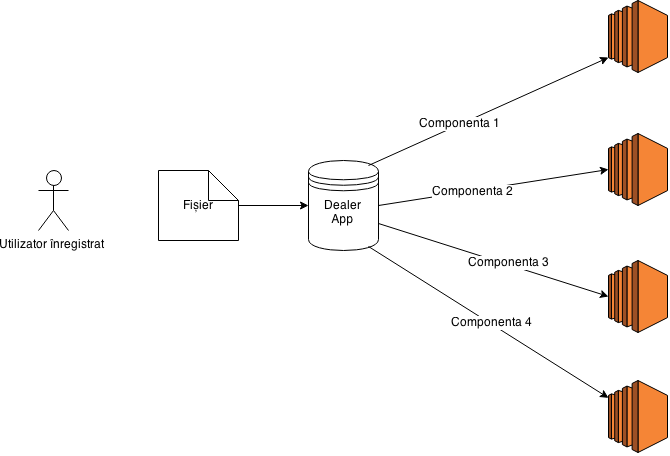
\includegraphics[width=1\textwidth]{img/DealerApp.png}
	\caption{Distribuirea unui fișier în DealerApp la $4$ instanțe EC2}
	\label{fig:dealerapp}
	\end{center}
	\bigskip
\end{figure}
%------------------------------------------------------------------------------------------
%------------------------------------------------------------------------------------------
%------------------------------------------------------------------------------------------
%------------------------------------------------------------------------------------------
%------------------------------------------------------------------------------------------
%------------------------------------------------------------------------------------------
% poate tehnologii folosite?
% About automatically startup scripts on EC2. AMI Images. Rest API, Django Framework, Angular
% Bootstrap, Bootswatch
\section{Tehnologii folosite}

\subsection{AWS}

\subsubsection{Boto}

\section{Redis}

\subsection{Django}

\subsubsection{Django REST Framework}
\label{subsub:rest}

\subsection{AngularJS}
\label{sub:angular}

\subsubsection{Twitter Bootstrap}

%------------------------------------------------------------------------------------------
%------------------------------------------------------------------------------------------
%------------------------------------------------------------------------------------------
%------------------------------------------------------------------------------------------
%------------------------------------------------------------------------------------------
%------------------------------------------------------------------------------------------
\section{Reconstituirea fișierelor}


%------------------------------------------------------------------------------------------
%------------------------------------------------------------------------------------------
%------------------------------------------------------------------------------------------
%------------------------------------------------------------------------------------------
%------------------------------------------------------------------------------------------
%------------------------------------------------------------------------------------------
%------------------------------------------------------------------------------------------

\clearpage

\bibliographystyle{splncs}
\bibliography{llncs}

\end{document}


